\documentclass[a4paper,12pt]{report}
% \usepackage[english]{babel}

% Set page size and margins
\usepackage[a4paper,top=2cm,bottom=2cm,left=2.5cm,right=2.5cm,marginparwidth=1.75cm]{geometry}

% Useful packages
\usepackage{amsmath,amssymb}
\usepackage{graphicx}
\usepackage{algorithm}
\usepackage{algpseudocode}
\usepackage{hyperref}
\usepackage{booktabs}
\usepackage{lscape}
\usepackage{longtable}
\usepackage{multicol}
\hypersetup{
    colorlinks=false,
    linkcolor=blue,
    filecolor=magenta,      
    urlcolor=cyan,
    pdftitle={World Trade Thesis},
    pdfpagemode=FullScreen,
    }
\usepackage[font=footnotesize]{caption}
\usepackage[dvipsnames]{xcolor}
\usepackage{setspace}
\doublespacing

% Citations
\usepackage[sorting=none, style=numeric, backend=biber]{biblatex}
\addbibresource{references.bib}
% \usepackage{fontspec}
% \setmainfont{Verdana}
% \renewcommand{\familydefault}{\sfdefault}

% \usepackage{csvsimple}


% Custom operators
%\DeclareMathOperator{\E}{\mathbb{E}}
% \DeclareMathOperator{\cal}[1]{\mathcal{#1}}
%\DeclareMathOperator{\fk}[1]{\mathfrak{#1}}
% \DeclareMathOperator{\bf}[1]{\mathbf{#1}}
%\DeclareMathOperator{\kl}[2]{KL \left( #1\,||\,#2 \right)}
%\newtheorem{definition}{Definition}[section]

\title{A Statistical Analysis of the World Trade Network}
\author{Pietro Dominietto}
\date{October 2022}



\begin{document}
\maketitle

% \begin{abstract}
% Abstract
% \end{abstract}

% \singlespacing
\begin{singlespace}

\tableofcontents

\listoftables
\listoffigures
\end{singlespace}
\pagebreak

% \doublespacing
% Introduction chapter
\chapter{Introduction chapter}

% ISTAT used a publicly available dataset (COMEXT, by Eurostat) which contains historical data about world imports and exports of goods since 2010, to gather insights and in the end produce a web tool to provide useful statistics and a graph visualization of the commerce network. 
The core idea of the research I've conducted is to construct a dataset about world import and exports of goods among world countries, to represent it as a directed graph and to produce insights about world trade using mathematical and statistical tools.
The inspiration for this work comes from the research internship I did with ISTAT (Italian National Institute of Statistics) and their previous research named \textit{Cosmopolitics}. % CITATION 
They used a publicly available dataset named COMEXT by \textcite{eurostat2022comext}, which contains, among other things, historical data about world imports and exports reported by EU countries, from 1988 until 2022. The project that they developed consisted in a web tool to provide useful statistics and a graph visualization of the European commerce network.\footnote{Tool online at  \href{https://cosmo.statlab.it/}{cosmo.statlab.it} Code available here \url{https://github.com/istat-methodology/cosmopolitics}}


\section{Research questions}

Now they are wondering what else could they exploit these data for:
\begin{itemize}
    \item Can we use the graph representation of the good exchanges to understand the commerce network and look at useful statistics of the graph, and how they relate to real world effects?
    \item[OLD] \textit{Starting from the graph representation of the commerce data, is it possible to train ML and NN methods (like GraphNN and Bayes Nets) to make predictions, evaluate scenarios and draw inferences on them?}
    \item Can we be able to build a model capable of learning how did commerce evolve through time and given the model be able to observe what changes happen in the system when we add, remove or modify a node or an edge?
    \item In fact, their research questions for my project are about using these data and the graphs generated to investigate whether it’s possible to apply ML and NN methods (like Bayesian Nets or GraphNNs) to draw inferences about the graphs and evaluate scenarios or compute forecasts.
\end{itemize}
% Data and Graphs chapter
%% TODO: in the chapter, better explain "the purpose of the analysis" once ch 2 is done

\chapter{From the Data to the Graphs}\label{ch:2data}
% mao bacini tantiii siiiiii
The goal of this chapter is to illustrate the data collection process and the procedures for data cleaning and integration that were undertaken. This part of the research is fundamental, since the validity of each following step depends on the reliability of the data that one is working with. In particular, the accuracy of any kind of insights and conclusions that one may draw about the networks and the scenarios that are observed is deeply rooted in the data gathering process.
Finding a unique and consistent data source for the purpose of this analysis was quite demanding, and in fact in the end I needed to combine information coming from multiple datasets. The following section will start by illustrating the multiple sources I have used including details and information about them, then I will move on into explaining the sequence of step I applied on the data to construct, in the end, the graphs and networks that are the base of my analysis.

\section{Data Sources}

The data needed for constructing the networks and performing the analysis come from multiple sources, and there are two main reasons for this: one is because the original dataset was incomplete about the world's trade network, and the second one is because, in order to be able to compare exchanges of different countries, I needed to have external exogenous variables that would give me additional information about the countries. In particular, the data sources that I employed are:
\begin{itemize}
    \item European Statistical Office (Eurostat) \cite{eurostat2022comext}, for the COMEXT dataset on European trade;
    \item World Trade Organization (WTO) \cite{wto2022stats}, for their dataset on global trade including non-EU countries;
    \item United Nations (UN) \cite{un2022population}, for the estimates of population that I used as exogenous variable;
    \item European Central Bank (ECB) \cite{ecb2021usdeur}, for the USD-EUR historical exchange rates that I needed to combine the datasets.
\end{itemize}

\subsection{COMEXT}

The starting dataset of my research is named COMEXT, and is published and maintained by Eurostat \cite{eurostat2022comext}. COMEXT is a statistical database for detailed statistics on international trade in goods\footnote{The definition of \textit{goods} provided by Eurostat is "\textit{all movable property including electricity}".}. It serves as an important indicator of the performance of the European Union (EU) economy, because it focuses on the size and the evolution of imports and exports of countries. It provides access not only to both recent and historical data of the EU and its individual Member States, but also to statistics of a significant number of non-EU countries. The information contained in it is based on data provided by the statistical agencies of the EU member states and trading partners.
Data are organized in tables, one for each year (or for each month) and each table contains information about the country that declared the transaction, the partner country, the product that was exchanged according to multiple international standard classifications (or nomenclatures), the value in euros of the exchange and its quantity in kilograms.
Let us now have a look at an extraction from this dataset, as you can see in Table \ref{tab:comextexample}.
The data available follow the shown format. Each row corresponds to a transaction, an exchange of a certain good between two countries in a given period. The information available about each transaction is summarized here:
\begin{itemize}
    \item \textit{DECLARANT} and \textit{DECLARANT ISO}: code and ISO\footnote{ISO stands for International Standardization Organization, which harmonizes codes and abbreviations across the world (\url{www.iso.org}). The conversion is displayed in Appendix Table \ref{tab:iso2}.} name of the country that declared the trade;
    \item \textit{PARTNER} and \textit{PARTNER ISO}: code and ISO name of the country with which the declarant traded;
    \item \textit{TRADE TYPE}: indicates whether the exchange was among two EU countries (I) or one was extra-EU (E);
    \item all the \textit{PRODUCT} columns: they are used to classify the good that was exchanged, according to different nomenclatures and standards;
    \item \textit{FLOW}: indicates whether the exchange was reported as an import (1) by the declarant or as an export (2);
    \item \textit{PERIOD}: indicates the time period of the exchange, in the format \texttt{yyyymm}\footnote{If it refers to a whole year then the format is \texttt{yyyy52}.};
    \item \textit{VALUE IN EUROS}: indicates the monetary value of the exchange between countries of that product;
    \item \textit{QUANTITY IN KG}: indicated the weight in kilograms of the exchange between countries of that product.
\end{itemize}
\begin{landscape}
\begin{table}
    \centering
    \resizebox{1.6\textheight}{!}{
\begin{tabular}{rrrrrrrrrrrrrrrrrrrr}
% \begin{tabular}{p{2.5cm}p{2.5cm}p{2cm}p{2cm}p{2cm}p{2cm}p{2cm}p{2cm}p{2cm}p{2cm}p{2cm}p{2cm}p{2cm}p{2cm}p{2cm}p{2cm}p{2cm}}
 \toprule
 DECLARANT & DECLARANT ISO & PARTNER & PARTNER ISO & TRADE TYPE & PRODUCT NC & PRODUCT SITC & PRODUCT cpa2002 & PRODUCT cpa2008 & PRODUCT CPA2 1 & PRODUCT BEC & PRODUCT SECTION & FLOW & PERIOD & VALUE IN EUROS & QUANTITY IN KG \\ \midrule
 61 & CZ & 4 & DE & I & 83023000 & 69915 & 2863 & 2572 & 2572 & 530 & 15 & 2 & 200101 & 284650 & 137370 \\
 5 & IT & 604 & LB & E & 85011010 & 71610 & 3110 & 2711 & 2711 & 410 & 16 & 2 & 200101 & 42089 & 11200 \\
 7 & IE & 5 & IT & I & 20021010 & 05672 & 1533 & 1039 & 1039 & 122 & 04 & 1 & 200101 & 97333 & 207000 \\
 4 & DE & 52 & TR & E & 85363030 & 77253 & 3120 & 2712 & 2712 & 420 & 16 & 2 & 200101 & 124054 & 3200 \\
 1 & FR & 720 & CN & E & 84823000 & 74630 & 2914 & 2815 & 2815 & 420 & 16 & 2 & 200101 & 18294 & 1300 \\
 30 & SE & 64 & HU & E & 72193310 & 67553 & 2710 & 2410 & 2410 & 220 & 15 & 2 & 200101 & 36002 & 18000 \\
 7 & IE & 720 & CN & E & 82089000 & 69561 & 2862 & 2573 & 2573 & 420 & 15 & 1 & 200101 & 15039 & 400 \\
 60 & PL & 1 & FR & I & 70091000 & 66481 & 2612 & 2312 & 2312 & 220 & 13 & 1 & 200101 & 12724 & 845 \\
 46 & MT & 400 & US & E & 85442000 & 77312 & 3130 & 2732 & 2732 & 220 & 16 & 1 & 200101 & 47203 & 0 \\
 30 & SE & 53 & EE & E & 62064000 & 84270 & 1823 & 1414 & 1414 & 620 & 11 & 1 & 200101 & 18944 & 500 \\
 1 & FR & 528 & AR & E & 90261099 & 87431 & 3320 & 2651 & 2651 & 410 & 18 & 2 & 200101 & 30657 & 500 \\
 3 & NL & 38 & AT & I & 28257000 & 52269 & 2412 & 2012 & 2012 & 220 & 06 & 2 & 200101 & 125073 & 20400 \\
 55 & LT & 5 & IT & I & 55103000 & 65187 & 1710 & 1310 & 1310 & 220 & 11 & 1 & 200101 & 26906 & 4033 \\
 5 & IT & 9 & GR & I & 84669195 & 72819 & 2940 & 2849 & 2849 & 420 & 16 & 2 & 200101 & 90529 & 5600 \\
 1 & FR & 4 & DE & I & 70140000 & 66595 & 2615 & 2319 & 2319 & 220 & 13 & 1 & 200101 & 410786 & 33400 \\
 5 & IT & 472 & TT & E & 94018000 & 82118 & 3611 & 3100 & 3100 & 410 & 20 & 2 & 200101 & 39182 & 25800 \\
 11 & ES & 75 & RU & E & 44091011 & 24830 & 2010 & 1610 & 1610 & 220 & 09 & 2 & 200101 & 27916 & 3000 \\
 61 & CZ & 3 & NL & I & 84807190 & 74918 & 2956 & 2573 & 2573 & 410 & 16 & 1 & 200101 & 167767 & 545 \\
 30 & SE & 39 & CH & E & 84563011 & 73113 & 2940 & 2841 & 2841 & 410 & 16 & 1 & 200101 & 295905 & 8500 \\
 32 & FI & 10 & PT & I & 48109190 & 64177 & 2112 & 1712 & 1712 & 220 & 10 & 2 & 200101 & 12252 & 13200 \\
 53 & EE & 54 & LV & E & 48229000 & 64291 & 2125 & 1729 & 1729 & 220 & 10 & 2 & 200101 & 14994 & 18678 \\
 6 & GB & 720 & CN & E & 84615011 & 73177 & 2940 & 2841 & 2841 & 410 & 16 & 1 & 200101 & 20997 & 1900 \\
 5 & IT & 60 & PL & E & 85189000 & 76492 & 3230 & 2640 & 2640 & 420 & 16 & 2 & 200101 & 250280 & 73200 \\
 5 & IT & 400 & US & E & 97020000 & 89620 & 9231 & 9003 & 9003 & 610 & 21 & 2 & 200101 & 12861 & 500 \\
 6 & GB & 61 & CZ & E & 84148079 & 74319 & 2912 & 2813 & 2813 & 410 & 16 & 2 & 200101 & 37962 & 2900 \\
 91 & SI & 5 & IT & I & 82074030 & 69564 & 2862 & 2573 & 2573 & 420 & 15 & 1 & 200101 & 17573 & 227 \\
 38 & AT & 92 & HR & E & 21032000 & 09842 & 1587 & 1084 & 1084 & 122 & 04 & 2 & 200101 & 17346 & 20200 \\
 1 & FR & 5 & IT & I & 39173231 & 58140 & 2521 & 2221 & 2221 & 220 & 07 & 1 & 200101 & 86548 & 29200 \\
 4 & DE & 52 & TR & E & 39173231 & 58140 & 2521 & 2221 & 2221 & 220 & 07 & 2 & 200101 & 75198 & 14400 \\
 6 & GB & 628 & JO & E & 84189990 & 74149 & 2923 & 2825 & 2825 & 420 & 16 & 2 & 200101 & 16498 & 10000 \\
 11 & ES & 4 & DE & I & 28129000 & 52241 & 2413 & 2013 & 2013 & 220 & 06 & 1 & 200101 & 17184 & 1800 \\
 8 & DK & 400 & US & E & 28183000 & 52266 & 2413 & 2013 & 2013 & 220 & 06 & 1 & 200101 & 140360 & 100000 \\
 4 & DE & 3 & NL & I & 82022000 & 69551 & 2862 & 2573 & 2573 & 420 & 15 & 1 & 200101 & 91395 & 3800 \\
 4 & DE & 63 & SK & E & 60012100 & 65512 & 1760 & 1391 & 1391 & 220 & 11 & 2 & 200101 & 48420 & 4200 \\
 92 & HR & 5 & IT & I & 94019080 & 82119 & 3611 & 3100 & 3100 & 220 & 20 & 1 & 200101 & 23887 & 10559 \\
 6 & GB & 8 & DK & I & 42029291 & 83199 & 1920 & 1512 & 1512 & 620 & 08 & 1 & 200101 & 73806 & 3100 \\
 11 & ES & 5 & IT & I & 85153100 & 73735 & 2940 & 2790 & 2790 & 410 & 16 & 1 & 200101 & 578296 & 29500 \\
 3 & NL & 386 & MW & E & 09024000 & 07414 & 0113 & 0127 & 0127 & 112 & 02 & 1 & 200101 & 97484 & 65000 \\
 17 & BE & 732 & JP & E & 39032000 & 57291 & 2416 & 2016 & 2016 & 220 & 07 & 1 & 200101 & 25108 & 5400 \\
 11 & ES & 3 & NL & I & 08103030 & 05794 & 0113 & 0125 & 0125 & 112 & 02 & 1 & 200101 & 16854 & 6200 \\
 1 & FR & 3 & NL & I & 72042900 & 28229 & 2710 & 3811 & 3811 & 210 & 15 & 2 & 200101 & 59015 & 258300 \\
 4 & DE & 979 & QZ & E & 29211930 & 51451 & 2414 & 2014 & 2014 & 220 & 06 & 2 & 200101 & 381600 & 372300 \\
 6 & GB & 17 & BE & I & 30021091 & 54163 & 2442 & 2120 & 2120 & 220 & 06 & 1 & 200101 & 4166599 & 1500 \\
 7 & IE & 6 & GB & I & 85421360 & 77641 & 3210 & 2611 & 2611 & 420 & 16 & 2 & 200101 & 438109 & 0 \\
 1 & FR & 640 & BH & E & 84431990 & 72659 & 2956 & 2899 & 2899 & 410 & 16 & 1 & 200101 & 41257 & 300 \\
 11 & ES & 3 & NL & I & 72193410 & 67554 & 2710 & 2410 & 2410 & 220 & 15 & 1 & 200101 & 118787 & 59300 \\
 7 & IE & 220 & EG & E & 84733090 & 75997 & 3002 & 2620 & 2620 & 420 & 16 & 2 & 200101 & 184452 & 1500 \\
 3 & NL & 388 & ZA & E & 90261051 & 87431 & 3320 & 2651 & 2651 & 410 & 18 & 2 & 200101 & 48644 & 900 \\
 1 & FR & 30 & SE & I & 84733010 & 75997 & 3002 & 2620 & 2620 & 420 & 16 & 2 & 200101 & 1138762 & 3800 \\
 60 & PL & 94 & YU & E & 16042090 & 03716 & 1520 & 1020 & 1020 & 122 & 04 & 2 & 200101 & 14171 & 9900 \\
 \bottomrule
\end{tabular}
}

    \caption{Random sample taken from the COMEXT dataset referring to imports and exports exchanged during January 2001.}
    \label{tab:comextexample}
\end{table}
\end{landscape}

\paragraph{Summary statistics}
Thanks to COMEXT data, we are able to conduct many types of analyses on commerce among countries. A first look at the data tells us that, by exploiting the variables that we have at disposal, we can observe if there are any trends in the EU economy as a whole, aggregating on all countries and products. This is shown in Figure \ref{fig:totaleu}. 

\begin{figure}
    \centering
    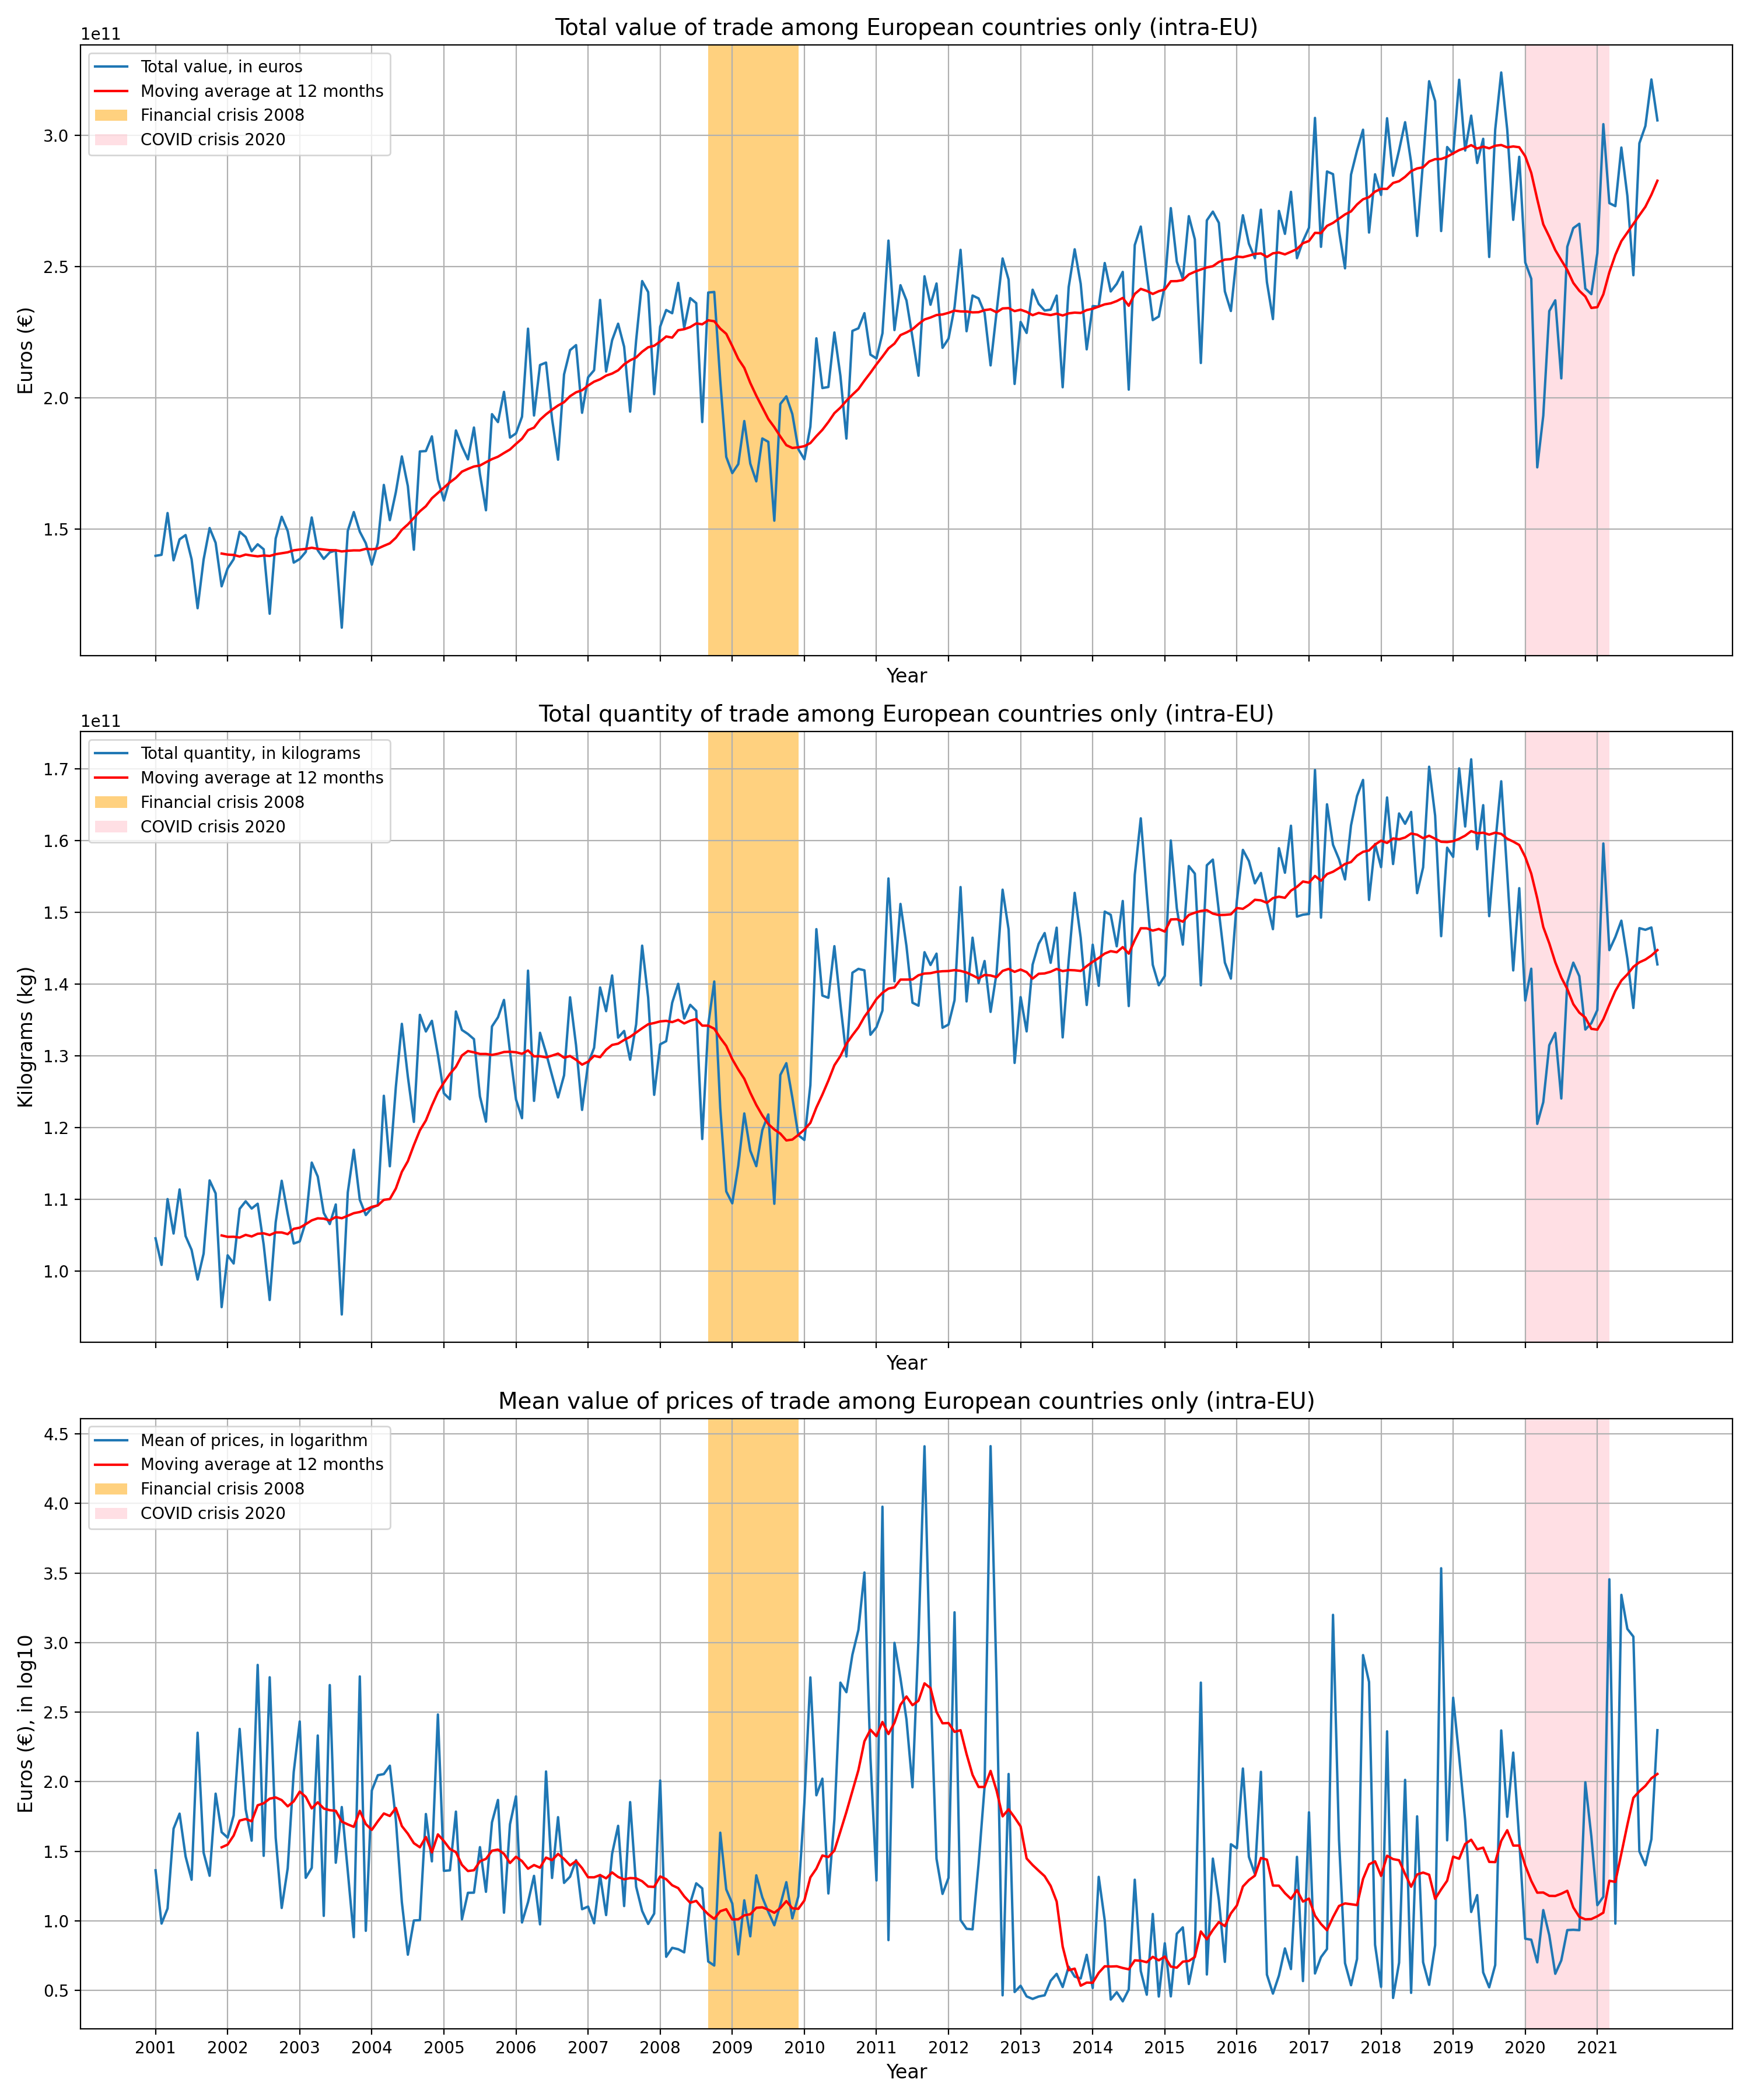
\includegraphics[width=\textwidth]{pics/TOTAL_VQP_INTRA.png}
    \caption[Long term trends of trade exchanges across EU member countries]{Long term trends of trade exchanges across EU member countries, by various indicators: (1) value (\texteuro), (2) quantity (Kg), (3) price (\texteuro/kg).}
    \label{fig:totaleu}
\end{figure}

In the first plot, we have on the horizontal axis time in years, while on the vertical axis we have monetary value expressed in euros. What is shown here is an aggregated sum of the total value of products exchanged by EU countries among themselves (intra-EU trade). This can be interpreted as an important indicator of the state of the whole economy, and in fact we can recognize in it two of the major economic events that happened in the last two decades: the 2008 financial crisis and the 2020 COVID-19 epidemic and related economic fallout. Since 2004 the growth of intra-EU trade was stable and sustained, up until the second semester of 2008, where we see a notable drop in total value, and a reprise only after the end of 2009. A similar effect can be seen at the beginning of 2020, where the lockdown due to the epidemic caused a sudden drop in the commerce of non-essential products, which almost brought the economy to a halt. Then production reprised in the second half of 2020, and we need to wait until 2021 for the values to reach pre-COVID levels.
If we look instead at the big picture, we see that overall intra-EU trade follows a positive trend that has basically doubled the value in 20 years. One has to wonder whether this increase in total money exchanged in commerce is due to an actual increase in production and circulation of goods, or is due just to inflation and higher prices of products. If we look at the second plot, we can observe the total quantity in kilograms of products exchanged in the EU economy. As before, we see a positive trend in the last 20 years, supporting our hypothesis that production has expanded. We also observe the same drops of trade exchanges following the two crises. Furthermore, what can be observed in both of the previous two plots is a yearly seasonality of these time series, where the values usually go up in the first trimester of the year, then they go down after mid-year, only to pick up again in the last part of the period. 
At last, in the third plot, we see the evolution of prices in the same time frame, obtained by dividing each exchange's value by its quantity. Note that the vertical axis is in log scale. Here we can see a different behavior than previously. While in the first eight years of the millennium prices of traded products have been going down, with less and less volatility year by year (which can also explain why demand and commerce of these goods has gone up), we can easily see that in the period following the 2008 crisis they went rapidly up again. This is a known and reasonable effect of those events, since, when dealing with scarcity and uncertainty, prices naturally rise, and with them also variability. It took more than three years after 2009 for these inflated prices to go down, and it can be easily seen that by the start of 2014 they were even lower than before 2008. Then they started slowly to grow, as we observe a  slight positive trend until 2020, with periodical cycles which last about a year. After 2021, which marked a first step out of the pandemic with the diffusion of COVID vaccines, we see the economy picking up again, and, as with the aftermath of crises, also prices and volatility increase.

%%esempio di tabella che viene da COMEXT -- altrimenti così son solo parole
%%Questo può essere quello che ti avevo segnato come capitolo 3 -- spiegazione etc etc 
%%Descrizione e visualizzazione del dataset - dati nulli, dati non comuni

\paragraph{COMEXT Data collection}
Historically, the main source of information about trade transactions between countries are customs authorities, which provide detailed information on exports and imports of goods with a geographical breakdown.
The COMEXT system was conceived and implemented in the early 90s,  following the adoption of the European Single Market in 1993, when customs formalities between Member States were removed. Since then, it has been continuously adapted and re-engineered to take into account technological evolution and new users' needs. The data gathered are based on two data collection systems:
\begin{itemize}
    \item data on trade in goods with non-EU countries are collected by customs authorities and are based on the records of trade transactions in customs declarations;
    \item data of intra-EU exchanges are directly collected from trade operators once a month.
\end{itemize}

The COMEXT dataset, however, presents a problem if one wants to use it to build an analysis on world trade. In fact, the only data contained in it are the ones reported by European countries, or even less than that, members of the European Union. Therefore, if we look at the whole network of commerce, we are missing some relevant information: the trade of extra-EU countries among themselves, since they have no obligation to communicate to Eurostat their records.
For this reason, and because I want to conduct a complete analysis and have a complete overview of the trade network, I needed to find another source of information, which I then integrated with COMEXT.

\subsection{WTO}
Similar to Eurostat, also the World Trade Organization (WTO) collects data about the global commerce of products among countries \cite{wto2022stats}. Data are periodically sent to the organization from member countries, hence the dataset contains information about all the major world countries.
Its structure is similar to COMEXT, but with a few differences: in fact, the data points are available with an annual periodicity instead of monthly as for the ones supplied by Eurostat. In Table \ref{tab:wtoexample} we can see a sample extracted from this dataset. As before, each row corresponds to the sum of exchanges between two countries in a given year, and for each import we have the following information:
\begin{itemize}
    \item \textit{Reporting Country}: the country that reported the value to WTO;
    \item \textit{Partner Country}: the country that exported the product to the reporting country;
    \item \textit{Product Code}: the code that identifies the category of the product exchanged, according to the Harmonized System (HS) nomenclature;
    \item \textit{Year}: indicating the year which the number refers to;
    \item \textit{Value}: the amount in US dollars that corresponds to the exchanged products' worth.
\end{itemize}

\begin{table}
    \centering
    \resizebox{1.0\textwidth}{!}{
\begin{tabular}{lllllr}
\toprule
 Reporting Economy Code & Partner Economy Code & Product Or Sector Code & Unit Code & Year & Value \\
\midrule
 356 & 826 & 970190 & USD & 2014 & 26972 \\
 268 & 840 & 961900 & USD & 2019 & 16323 \\
 716 & 840 & 970110 & USD & 2011 & 1613 \\
 800 & 840 & 960990 & USD & 2010 & 1126 \\
 344 & 826 & 960899 & USD & 2010 & 399676 \\
 634 & 784 & 961800 & USD & 2017 & 42030 \\
 716 & 800 & 970110 & USD & 2013 & 15 \\
 050 & 840 & 960839 & USD & 2008 & 424 \\
 410 & 840 & 970500 & USD & 2016 & 1929898 \\
 048 & 840 & 961210 & USD & 2004 & 45543 \\
 124 & 840 & 961511 & USD & 2009 & 684780 \\
 076 & 840 & 961210 & USD & 2002 & 2689590 \\
 410 & 764 & 970300 & USD & 2014 & 448973 \\
 800 & 840 & 970110 & USD & 2016 & 424 \\
 454 & 840 & 961610 & USD & 2006 & 326 \\
 376 & 840 & 960899 & USD & 2013 & 25000 \\
 840 & 862 & 960920 & USD & 2005 & 161269 \\
 600 & 840 & 960899 & USD & 2015 & 2542 \\
 756 & 784 & 970190 & USD & 2013 & 947 \\
 807 & 840 & 960910 & USD & 2001 & 100 \\
 458 & 840 & 961320 & USD & 2002 & 71548 \\
 834 & 792 & 960990 & USD & 2010 & 3 \\
 646 & 800 & 960899 & USD & 2018 & 17 \\
 352 & 764 & 961590 & USD & 2008 & 294 \\
 344 & 804 & 961800 & USD & 2013 & 50 \\
 222 & 840 & 962000 & USD & 2019 & 25475 \\
 124 & 764 & 961220 & USD & 2014 & 74935 \\
 702 & 764 & 961220 & USD & 2010 & 4077 \\
 268 & 784 & 960850 & USD & 2007 & 1200 \\
 356 & 826 & 961390 & USD & 2015 & 68 \\
 454 & 834 & 961700 & USD & 2013 & 3275 \\
 268 & 792 & 961390 & USD & 2005 & 1000 \\
 410 & 840 & 960850 & USD & 2007 & 4072 \\
 124 & 764 & 960910 & USD & 2009 & 507329 \\
 554 & 704 & 960910 & USD & 2012 & 219 \\
 156 & 704 & 970190 & USD & 2006 & 130 \\
 036 & 826 & 961320 & USD & 2006 & 4602 \\
 586 & 840 & 960860 & USD & 2004 & 6731 \\
 148 & 784 & 961590 & USD & 2012 & 3946 \\
 800 & 826 & 961511 & USD & 2016 & 6735 \\
 417 & 764 & 960910 & USD & 2017 & 1055 \\
 188 & 826 & 961000 & USD & 2005 & 10 \\
 792 & 840 & 961220 & USD & 2020 & 4682 \\
 616 & 792 & 961700 & USD & 2003 & 107 \\
 454 & 840 & 960990 & USD & 2008 & 208 \\
 764 & 704 & 960840 & USD & 2017 & 75 \\
 152 & 840 & 970400 & USD & 2001 & 1471 \\
 756 & 840 & 960891 & USD & 2020 & 3212 \\
 918 & 704 & 960899 & USD & 2001 & 3233 \\
 858 & 840 & 961610 & USD & 2008 & 3766 \\
\bottomrule
\end{tabular}
}
    \caption[Random sample taken from the WTO dataset]{Random sample taken from the WTO dataset, including codes of the HS nomenclature ranging from 960000 to 970000.}
    \label{tab:wtoexample}
\end{table}

Given the two available datasets, I had to find a way to combine them and to merge the variables of one with the other. Specifically, I needed to solve the following issues:
\begin{enumerate}
    \item The information about the European countries was repeated in both datasets, so it was necessary to choose which one to keep;
    \item The nomenclature for the products was different, so I used a conversion table and transformed one into the other;
    \item The monetary value of the exchange was in US dollars, so I converted it to Euros according to the exchange rate of that period.
\end{enumerate}

Hence, I proceeded as follows. For issue (1) I decided to keep the data from COMEXT and integrate them with WTO: this means that if we partition the countries in EU members and non-EU members, I get from COMEXT the data on intra-EU trade plus trade where one of the two countries is an EU member\footnote{More specifically, being an EU member for this purpose means that in that year the country has declared their numbers to Eurostat.}, while I get from WTO the rest of the trade data, that is, exchanges among two extra-EU countries.
Regarding issue (2), the solution was straightforward once I employed a conversion table, that allowed me to go from the HS classification to the CPA 2.1 nomenclature, as explained in Section \ref{sec:nomandusd}, while, for issue (3), in the same Section I'll show how the values were converted from US dollars to Euros, using a variable annual exchange rate.


\subsection{Nomenclatures and Currency}\label{sec:nomandusd}

In order to classify products into categories, many nomenclatures (or classifications) have been published by different organizations. Product classifications are designed to categorize products that have common characteristics. They provide the basis for collecting and calculating statistics on the production, distributive trade, consumption, international trade and transport of such products. The two datasets that I want to integrate, COMEXT and WTO, follow two different nomenclatures, created by two different institutions.
One of them is the Classification of Products by Activity (CPA), maintained by the European Commission and Eurostat.
According to Eurostat \cite{eurostat2022website}, "\textit{a statistical classification or nomenclature is an exhaustive and structured set of mutually exclusive and well-described categories, often presented in a hierarchy that is reflected by the numeric or alphabetical codes assigned to them, used to standardize concepts and compile statistical data}".
This procedure ensures that data is comparable between EU Member States, and for the purposes of this research, it enables us to put together reports of exchanges declared by different countries. While products in COMEXT are classified according to CPA, in the WTO dataset they follow the Harmonized Commodity Description and Coding System (HS), developed by the World Customs Organization (WCO) \cite{wco2022hs}. The system is used by more than 200 countries and economies as a basis for their Customs tariffs and for the collection of international trade statistics.\\
Although they have different categories and codes, these two nomenclatures have the same hierarchical structure: the classification starts with a super-category which is then broken down into smaller subcategories, adding more details to the description. This is highlighted by the digits or couple of digits of the numerical code that identifies the product. As an example, let us take the first row of Table \ref{tab:comextexample}, which is from COMEXT. The code in the column for CPA 2.1 is ``2572", and it is read in the following way:
\begin{itemize}
    \item The first two digits identify the broader category: in this case ``25" corresponds to \textit{Fabricated metal products, except machinery and equipment};
    \item The third digit identifies the first subcategory: ``257" corresponds to \textit{Cutlery, tools and general hardware};
    \item The fourth digit identifies the second subcategory: ``2572" corresponds to \textit{Locks and hinges}.
\end{itemize}
The analysis that will be conducted will focus only on the super-categories, that are identified by the first two digits of the code. The motivation behind this is that such classification is specific enough to be able to identify a relevant trade marked for these goods, but not too detailed so to fall into niche markets.
Therefore, before integrating the two data sources, what I needed to do was to convert the codes from the HS nomenclature in the WTO dataset into codes from the CPA 2.1, thanks to conversion tables provided by Eurostat\footnote{Available at \url{https://ec.europa.eu/eurostat/ramon/index.cfm} .}.

% PLOT WITH MAIN CATEGORIES
% TABLE WITH TWO DIGIT CPA CATEGORIES IN APPENDIX

% \paragraph{Currency exchange}\label{sec:usdeur}
The last issue to deal with when integrating the data is the change of currency, as I wanted to compare everything in euros. Since my purpose is to compare trade over time, I could not use a single value for the exchange rate. Hence, I used the dataset provided by the European Central Bank \cite{ecb2021usdeur}, which reports the weekly value of the exchange rates, as well as the annual value. The numbers I used are shown in Table \ref{tab:usdeur}.

\begin{table}
    \centering
    \begin{tabular}{lc||lc}
\toprule
Year & EUR / USD & Year & EUR / USD \\
\midrule
2001 & 0.8956 & 2012 & 1.2848 \\
2002 & 0.9456 & 2013 & 1.3281 \\
2003 & 1.1312 & 2014 & 1.3285 \\
2004 & 1.2439 & 2015 & 1.1095 \\
2005 & 1.2441 & 2016 & 1.1069 \\
2006 & 1.2556 & 2017 & 1.1297 \\
2007 & 1.3705 & 2018 & 1.1810 \\
2008 & 1.4708 & 2019 & 1.1195 \\
2009 & 1.3948 & 2020 & 1.1422 \\
2010 & 1.3257 & 2021 & 1.1827 \\
2011 & 1.3920 & & \\
\bottomrule
\end{tabular}
    \caption{ECB's annual exchange rates from USD to EUR.}
    \label{tab:usdeur}
\end{table}


\section{Towards the Network}

Once I have dealt with the change of nomenclature and currency, I can now merge the two data sources together to obtain a unique dataset and use it as starting point of my analysis. In this section, I will proceed to construct networks upon this dataset with countries as nodes and trades as edges. 

% 1 Mischio I/E
\subsection{Combining the Flows}
In order to proceed with the construction of the graphs, I needed to address a necessary adjustment to adopt regarding the COMEXT dataset. In fact, each EU country periodically sends information to Eurostat regarding the products traded and the amounts of both imports and exports. Therefore, if we take two countries that are both EU members, we will find four data entries of exchanges between them in a given period, although they refer to just two different exchanges (import and export). To better understand, we can look at Table \ref{tab:flows}. The first row displays the imports (flow equal to 1) of France from Germany of the product 3030, and this exchange was declared by France. Since they are both in the EU, we should expect also to have an entry of the same product declared by Germany but reported as export (flow equal to 2), and in fact we see it in row 3. The same goes for the opposite direction of the trade, from France to Germany, and in fact we find it in rows 2 and 4. The issue with this is that the numbers reported are not the same, but we encounter some discrepancy. Sometimes the difference is negligible, while other times it is more significant. For example, in this case the difference between what was declared by France and by Germany can account for a relative error of $13.3\%$. One possible reason why this is the case might have to do with the timing at which countries report their numbers, due to transportation times, delays, or simple bureaucratic procedures. For example, an exchange might be reported under one month for a country and under the following one for the other country.
Independently of the reason, I decided to proceed by averaging the two numbers. The rationale behind this is that for the purposes of my analysis, the relevant information is the relative size of this trade relationship with respect to other countries or to other products, and by taking the average I still maintain the same order of magnitude and size of the transaction.
Therefore, once I have grouped the rows in pairs and averaged them, I can proceed to the next step of the data preparation.

\begin{table}[h]
    \centering
    % \resizebox{1.0\textwidth}{!}
    {\small
    \begin{tabular}{l|llrrrr}
\toprule
 & DECLARANT & PARTNER & CPA 2.1 & FLOW & VALUE € & QUANTITY Kg \\
\midrule
1 & FR & DE & 3030 & 1 & 998489363 & 1382900 \\
2 & FR & DE & 3030 & 2 & 966169449 & 1364000 \\
3 & DE & FR & 3030 & 2 & 881409845 & 1304400 \\
4 & DE & FR & 3030 & 1 & 864220804 & 987500 \\
5 & DE & IT & 2910 & 2 & 813715037 & 74684600 \\
6 & FR & DE & 2910 & 1 & 733060859 & 70374600 \\
7 & IT & DE & 2910 & 1 & 670018217 & 69451300 \\
8 & DE & FR & 2910 & 2 & 649603453 & 62301400 \\
9 & FR & IT & 2910 & 2 & 321173553 & 39932800 \\
10 & IT & FR & 2910 & 1 & 316036092 & 38002800 \\
11 & FR & IT & 3030 & 1 & 252268490 & 402900 \\
12 & IT & FR & 2910 & 2 & 216223305 & 27218400 \\
\bottomrule
\end{tabular}

    }
    \caption[Example of double data entries for the same exchange in January 2001 in the COMEXT dataset, filtered only for IT, DE, FR.]{Example of double data entries for the same exchange in January 2001 in the COMEXT dataset, filtered only for IT, DE, FR. The codes of the product shown refer to: 3030: \textit{Air and spacecraft and related machinery}; 2910: \textit{Motor vehicles}.}
    \label{tab:flows}
\end{table}

% 2 Normalize
\subsection{Normalizing by Population}
Being able to produce aggregate statistics, is just the starting point of one's analysis. Given the data at hand, one would want to be able to confront the imports and exports of different countries and be able to tell which exchanges are most relevant to a nation's economy. However, every country has different size, and, with it, different expenses of the economy, different levels of production and needs for importing products that can't in any way be self produced. For example, small countries such as Luxembourg, Vatican City, San Marino have very high import expenses relatively to their size, while larger countries such as Germany, France or Italy may present a bigger number in absolute value, but it may constitute a small part of the country's economy.
Therefore, to be able to confront these types of exchanges, I needed to find an exogenous normalizing variable, which would serve as a proxy of the country's size of the economy, and would provide me with an indicator of each exchange's importance for the receiving country. 
In my analysis, I chose to use the country's population. I used the data published by the United Nations, as part of the 2022 Revision of the World Population Prospects \cite{un2022population} (curated by the Population Division of the Department of Economic and Social Affairs of the United Nations Secretariat). It presents population estimates from 1950 to the present for 237 countries, as well as population projections to the year 2100, which however are not of interest in this research. The table contains population data for each country for each year, and a reduced version is presented in Appendix \ref{app:unpop}, showing the numbers every 5 years.
What I would do then is to take, for each row of the dataset (as in Tables \ref{tab:comextexample} and \ref{tab:wtoexample}), the variable of the monetary value (and weight) and divide them by the population of the receiving country in that year. 

\begin{table}[t]
    \centering
    \resizebox{1.0\textwidth}{!}{
\begin{tabular}{llrrrrr}
\toprule
country from & country to & VALUE € & Q.TY Kg & population & VALUE € SCALED & Q.TY Kg SCALED \\
\midrule
 PT & GB & 3062165199 & 1850491617 & 67059.474 & 45663.42 & 27594.78 \\
 SA & TR & 1451527517 & 0 & 84135.428 & 17252.27 & 0.00 \\
 TN & DE & 1429474275 & 162837074 & 83328.988 & 17154.58 & 1954.14 \\
 RO & SG & 47640967 & 38817719 & 5909.869 & 8061.25 & 6568.28 \\
 QA & IN & 6942816036 & 0 & 1396387.127 & 4971.98 & 0.00 \\
 CZ & EG & 381686554 & 54100942 & 107465.134 & 3551.72 & 503.42 \\
 LV & BA & 3722674 & 2246260 & 3318.407 & 1121.82 & 676.90 \\
 LT & VN & 19320489 & 25798511 & 96648.685 & 199.90 & 266.93 \\
 SK & SR & 23211 & 24952 & 607.065 & 38.23 & 41.10 \\
 VU & IT & 21535 & 15000 & 59500.579 & 0.36 & 0.25 \\
\bottomrule
\end{tabular}
}
    \caption[Random sample of exchanges from 2021 taken from the combined COMEXT-WTO dataset]{Random sample of exchanges from 2021 taken from the combined COMEXT-WTO dataset. The numbers refer to the totality of products imported from that country in that year, the population in expressed in thousands.}
    \label{tab:normexample}
\end{table}

A sample of the resulting normalization is shown in Table \ref{tab:normexample}. If we look at the first row, we have there reported the total value of imports from Portugal (PT) to the United Kingdom (GB) in 2021, and it amounts to around 3 billion euros worth of products. In order to assess whether this is an important expenditure for the UK, we divide this number by the estimated population of Great Britain in 2021, i.e. around 67 million people, and we get an expense of 45,663 euros for every 1000 citizens. The same is done for the other rows, and this produces a variable that we can compare both across countries and across years, since we take into account population's evolution through time. As an example of why normalization is fundamental, we can have a look at row 5, that is, imports from Qatar (QA) to India (IN). The absolute value of the exchanged products' worth is more than double the one between PT and GB, however, since India has a population of almost 1.4 billion people (which is more than twenty times the population of the UK) the resulting normalized variable has a value which is ten times less than the one in the first row. Looking at the two relationships between the four countries, my interpretation is that, for the UK, the imports from Portugal can be considered more important than the imports from Qatar are for India. Or in other words, we can say that the dependence of the UK from Portugal is stronger than the dependence of India from Qatar. This type of comparison gains more meaning when comparing imports of the same product, implying a stronger expense pro capite of that good, or imports/exports from the same country or to the same country. For example we can see which are the main import or export partners of Italy, by ranking them according to this normalized variable (Table \ref{tab:itIEtop10}).\\
Hence, as a result of this normalization, I have created a variable which is relevant for what I am going to do next, that is building a graph where the nodes are the countries and the links are the exchanges of products, weighted with this new variable.

\begin{table}
    \centering
    \resizebox{1.0\textwidth}{!}{
    \begin{tabular}{llrrrrr}
\toprule
Country from & Country to & VALUE € & Q.TY Kg & Population & VALUE € SCALED & Q.TY Kg SCALED \\
\midrule
 DE & IT & 75490802662 & 21364308622 & 59240.329 & 1274314.372 & 360637.913 \\
 FR & IT & 39318792743 & 15193672582 & 59240.329 & 663716.651 & 256475.155 \\
 CN & IT & 38524642760 & 6459833416 & 59240.329 & 650311.087 & 109044.523 \\
 NL & IT & 29958184669 & 8229757030 & 59240.329 & 505705.913 & 138921.528 \\
 ES & IT & 25855033335 & 11269613640 & 59240.329 & 436443.108 & 190235.501 \\
 BE & IT & 21549565065 & 5314351392 & 59240.329 & 363765.115 & 89708.337 \\
 RU & IT & 17597932037 & 39156394849 & 59240.329 & 297059.998 & 660975.310 \\
 US & IT & 15810270013 & 8125519333 & 59240.329 & 266883.562 & 137161.955 \\
 PL & IT & 12536752795 & 3704847066 & 59240.329 & 211625.307 & 62539.272 \\
 CH & IT & 11147316509 & 1655703488 & 59240.329 & 188171.077 & 27948.925 \\
\midrule
 IT & VA & 56921605 & 10461387 & 0.511 & 111392573.386 & 20472381.605 \\
 IT & GI & 1001004532 & 2143793766 & 32.669 & 30640807.248 & 65621652.515 \\
 IT & KY & 474127906 & 3281377 & 68.136 & 6958552.102 & 48159.226 \\
 IT & MH & 213689418 & 137891 & 42.050 & 5081793.532 & 3279.215 \\
 IT & VG & 134370496 & 337436 & 31.122 & 4317540.518 & 10842.362 \\
 IT & CH & 27251973254 & 4407077721 & 8691.406 & 3135508.024 & 507061.541 \\
 IT & MT & 1472661244 & 1717929987 & 526.748 & 2795760.485 & 3261388.723 \\
 IT & SI & 4612331986 & 3143143021 & 2119.410 & 2176233.946 & 1483027.362 \\
 IT & BE & 17809938868 & 4324903577 & 11611.419 & 1533829.661 & 372469.857 \\
 IT & SM & 45241094 & 37063680 & 33.745 & 1340675.478 & 1098345.829 \\
\bottomrule
\end{tabular}
    }
    \caption[List of top Italy's top 10 trade partners.]{List of top Italy's top 10 trade partners, first for imports then for exports.}
    \label{tab:itIEtop10}
\end{table}



% 3 Creo grafo pesato (nodi poi archi)
\subsection{Creating the graphs}\label{sec:ch3graphs}
% TODO: why value and not quantity
Once I have normalized the values and reduced the rows to contain unique information, I am left with a unique dataset with the following information on the columns:
\begin{itemize}
    \item \textit{Year}: indicating the period which the values refer to;
    \item \textit{Country From}: indicating the country where the product originated from;
    \item \textit{Country To}: indicating the country where the product went to;
    \item \textit{Product Code}: indicating the category of the product according to the CPA 2.1 nomenclature;
    \item \textit{Normalized Value}: indicating the normalized expense for that import, expressed in \texteuro per 1000 inhabitants.
\end{itemize}
International trade is often referred to as a network, and in fact it is quite straightforward to represent it as a graph. Given the year we want to focus on, we can consider as nodes the countries of the world, and then we can add edges between them based on whether they are trade partners or not. This is the simplest network that can be constructed, and using this basic schema, we can construct different types of graphs. As a matter of fact, the main part of the analysis will deal with \textit{directed weighted networks}: the connections between nodes have a weight and a direction, from one node to the other. The weights of the edges are assigned according to the normalized value of the expense for that product in a specific year, and the direction of the exchange will go from the country that exports to the country that imports, following the same movement that the merchandise does in reality.
As an example, we can have a look at Figure \ref{fig:gcomext}, where we can observe the entire trade network of European countries (in blue) among themselves and also with extra-EU partners (in red). The layout of the graph helps us understand some characteristics of the network: nodes with more edges and with higher weight are attracted to each other, as we clearly see with the dense web of trade among European countries. Instead, the nodes which have weaker links tend to stay more at the periphery of the network, engaging less in trading activities with other countries. However, this particular representation is biased, since we lack a relevant block of information. We can directly observe the problem with COMEXT data alone that was exposed before: since there is no information in this dataset about trade among non-EU countries, it is hard to have a comprehensive view of the whole network of exchanges. 
In fact, one of the world's strongest economies and renowned center of global trade, the United States, is placed in a minor position in this layout, which doesn't reflect reality. If instead we integrate the data with the information from WTO, then we can complete the network and what we obtain is shown in Figure \ref{fig:gcomplete}. To help better underline how many trade edges were missing from the previous graph, here the exchanges among extra-EU countries are shown in \textit{azure}. This is the type of network which I'll base my analysis on, since it allows for a mathematical representation of the data which gives rise to many useful statistics, as it will be detailed in the next chapter.
\pagebreak
\begin{figure}[H]
    \centering
    \includegraphics[width=0.9\textwidth]{pics/full_y19_p10_5.png}
    \caption[Example of the trade network of from COMEXT data.]{Example of trade network with COMEXT data, showing the exchanges of \textit{Food Products}. The color of the node indicates EU countries (\textit{blue}) and non-EU (\textit{red}); the color of the edge is \textit{orange} for intra-EU exchanges, \textit{pink} for EU - non-EU exchanges.}
    \label{fig:gcomext}
\end{figure}
\begin{figure}[H]
    \centering
    \includegraphics[width=0.9\textwidth]{pics/complete_y19_p10_6.png}
    \caption[Example of trade network with COMEXT and WTO data.]{Example of trade network with COMEXT and WTO data, showing the exchanges of \textit{Food Products}. The color of the node indicates EU countries (\textit{blue}) and non-EU (\textit{red}); the color of the edge is \textit{orange} for intra-EU exchanges, \textit{pink} for EU - non-EU exchanges and \textit{azure} for extra-EU exchanges.}
    \label{fig:gcomplete}
\end{figure}


% 4 Threshold per rete binaria
\subsection{Binarizing the graph}\label{sec:3binarygraphs}
Another possibility instead of building a weighted graph is to use a threshold rule to decide whether two countries have a link connecting them or not. The new \textit{binary undirected} network obtained in this way, provides us with a way to treat the exchanges all in the same way, and shifts the focus of the methods and the analysis on the trade partnerships rather than on the amount of traded goods. The delicate part however is the choice of the numerical threshold below which one would not add a connection between two countries. To do so, it is important to first have a look at the distribution of the value in euros of the imports and exports. This can be seen in Figure \ref{fig:distrfood19}. 
The first thing that this distribution plot can tell us is that the monetary values of the exchanges approximately follows a log-normal distribution, that is to say that the distribution of the logarithm of these values (which is what is shown in the figure) resembles the Gaussian distribution, although it has a left tail heavier than the right. If we look at the numbers of this left tail, we see that a big part of them lies below 0 in log, which is equivalent to expenditures of 1 euro per 1000 people.
In my opinion, such an expense for a country can be neglected, especially since others spend up to $10^6$ \textit{euros / 1000 people} and even more. Thus, I wanted to find a threshold that would separate the data eliminating the lowest values, and I proceeded as follows. Instead of imposing the numerical value as an assumption, I computed the threshold such that, for each category, if we consider the entire world expense per 1000 inhabitants, then the values higher than such threshold would account for $99.999\%$ of this expenditure. This threshold rule would allow me to cut the lowest trade exchanges, including those that were the result of reporting errors present in the original datasets. Therefore, we can consider the complete trade network of \textit{Food Products} from the combined COMEXT-WTO dataset and we can apply the threshold to produce a binary network, which is shown in Figure \ref{fig:foodbingraph}.
\begin{figure}[h]
    \centering
    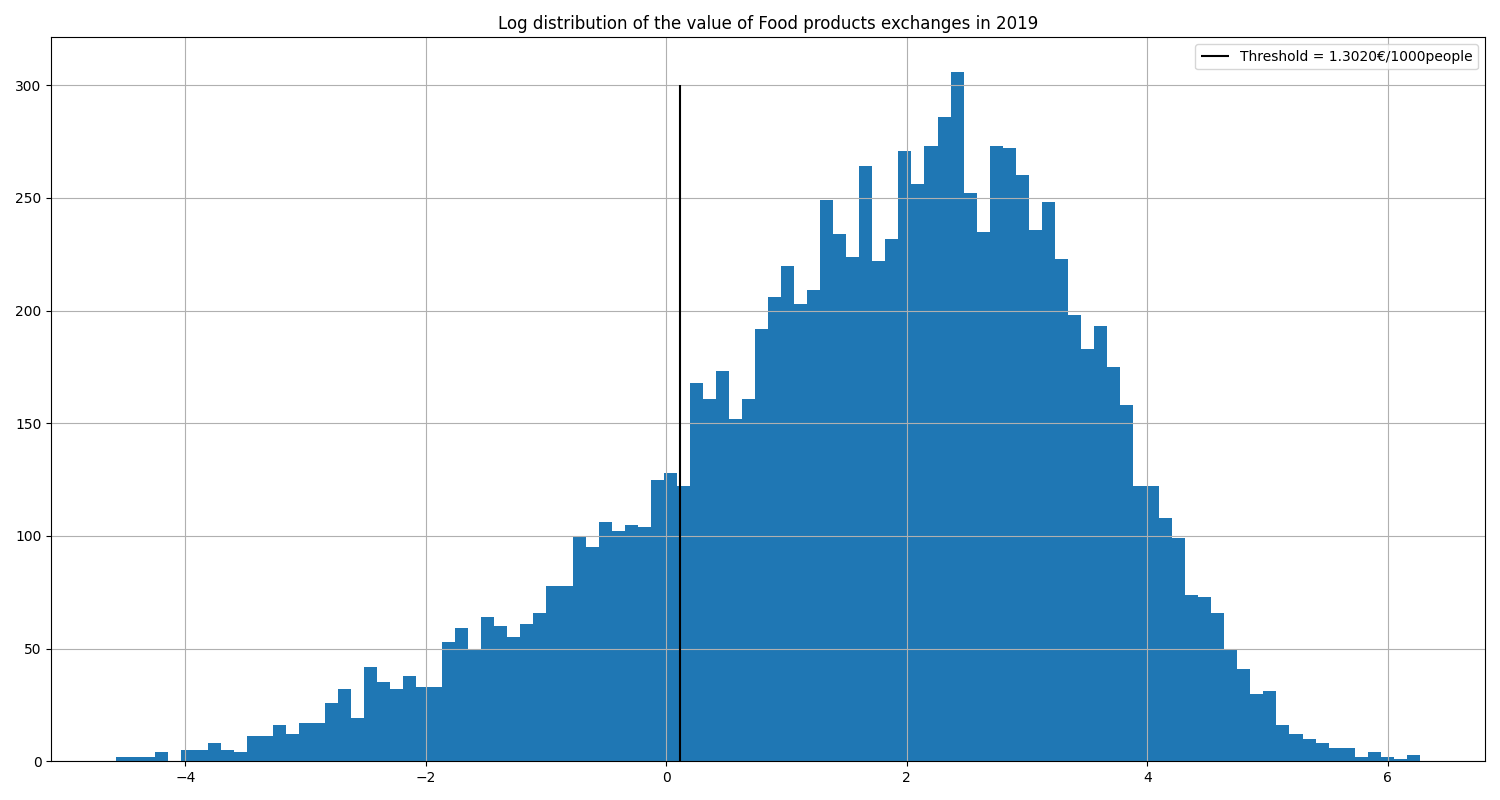
\includegraphics[width=\textwidth]{pics/thresh_complete_y19_p10.png}
    \caption{Distribution of the value of exchanges for the trade network of Food Products in 2019.}
    \label{fig:distrfood19}
\end{figure}

\begin{figure}
    \centering
    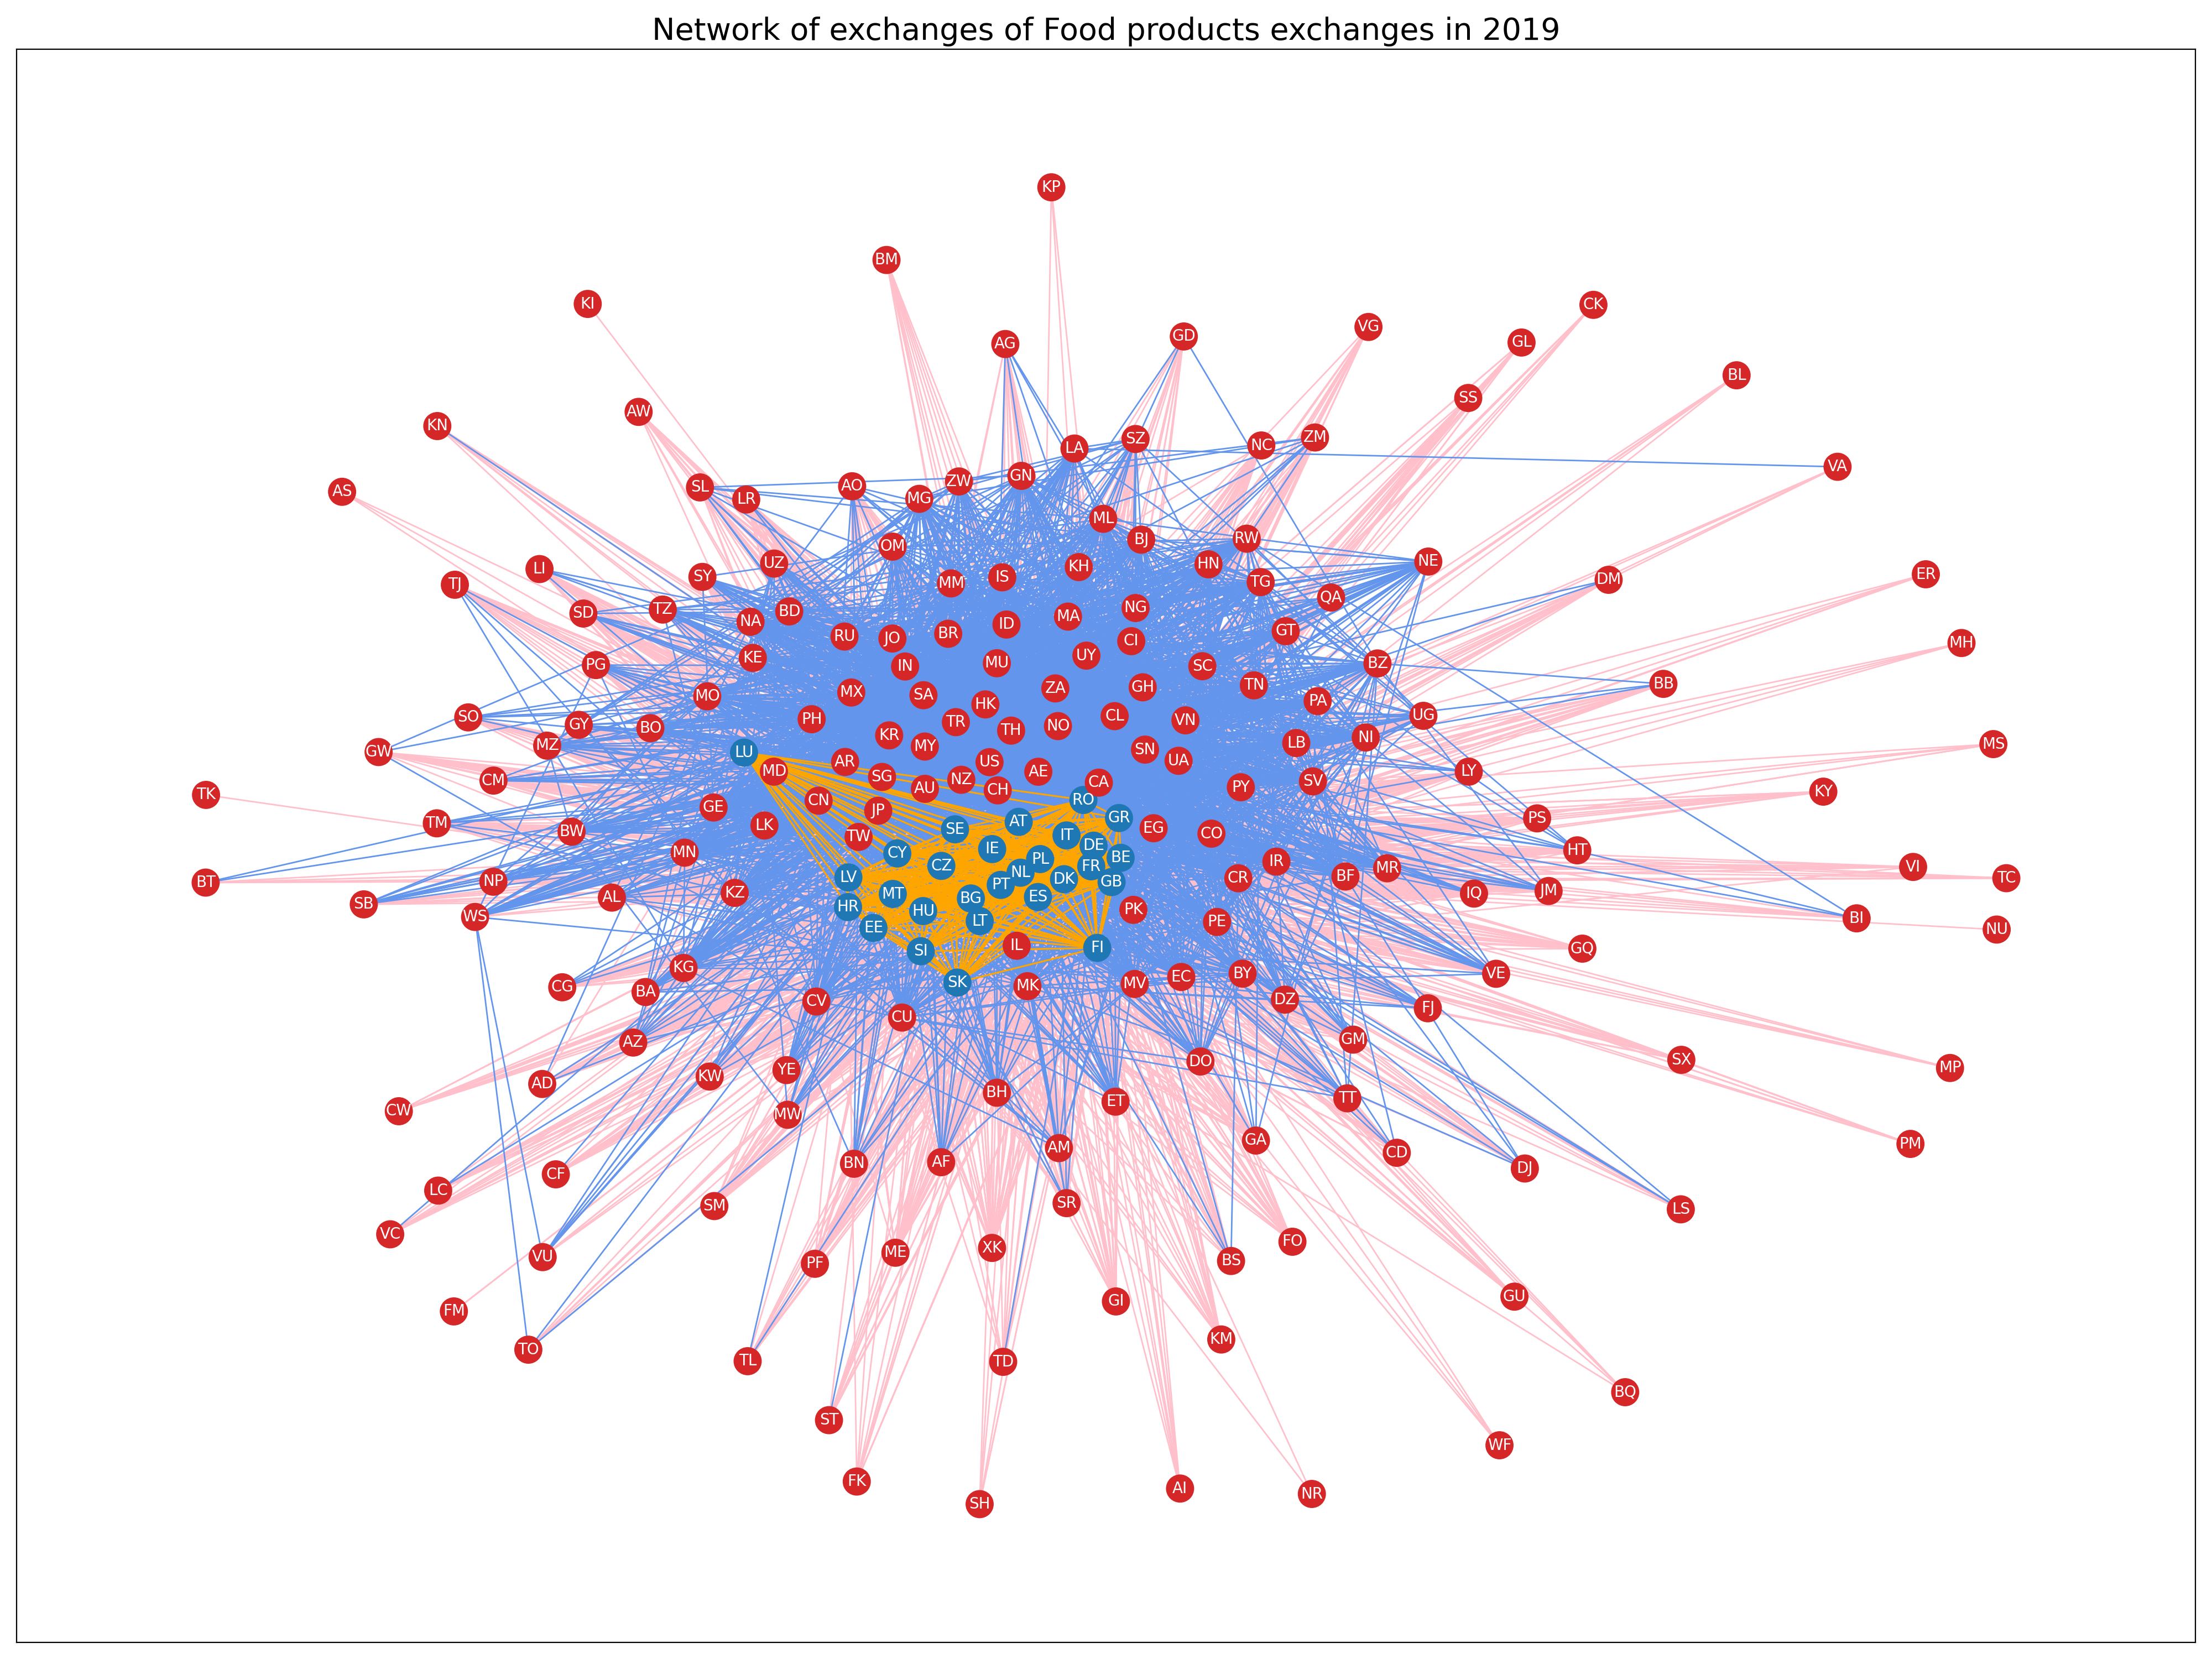
\includegraphics[width=\textwidth]{pics/complete_y19_p10_bin_7.png}
    \caption[Trade network of \textit{Food Products} in 2019, represented as a binary graph.]{Trade network of \textit{Food Products} in 2019, represented as a binary undirected graph using $1.302$ €/1000people as threshold. The color of the node indicates EU countries (\textit{blue}) and non-EU (\textit{red}); the color of the edge is \textit{orange} for intra-EU exchanges, \textit{pink} for EU - non-EU exchanges and \textit{azure} for extra-EU exchanges.}
    \label{fig:foodbingraph}
\end{figure}
% Methods chapter
\chapter{Methods for Network Analysis}\label{ch:3methods}

In the current chapter, I will explore the mathematical and statistical techniques that are behind my analysis of the world trade networks. In order to better understand the results that I will show in the next chapter, it is essential to have an understanding not only of the basic concepts of graph theory, but also of the mechanisms and dynamics of the statistical tools that I employ, from the simplest to the more elaborated. I will start by introducing what is a graph (Sec. \ref{sec:4graphtheory}), what are its properties, which metrics we can look at to study it and how we can visualize it to gain knowledge from the plots (Sec \ref{sec:4visualization}). Then I will continue by expanding more on the relevant techinques used for Network Analysis, by presenting the ideas of PageRank, hubs and authorities, and the methods to compute them (Sec. \ref{sec:4pagerank}). Lastly, I will talk about an additional query that one can do on a graph, that is community detection (Sec \ref{sec:4community}): I will explain two methods, Louvain and Stochastic Block Model, that allow one to look for possible communities in graphs, that is to say groups of nodes with similar behavior, like for example a limited group of countries that trades only among them. The following surveys of the statistical techniques I decided to use are adapted from \textcite{barabasi2016network,easley2012networks}.

\section{Intro to Graph Theory}\label{sec:4graphtheory}

If we want to understand a complex system, we first need to know how its components interact with each other or, in other words, we need a map of its wiring diagram.
Let us start by defining formally what is a graph, since it is fundamental for the analysis that will be carried out. 
A \textit{graph} is a way of specifying relationships among a collection of items. It consists of a set of objects, called \textit{nodes}, with certain pairs of these objects connected by links called \textit{edges}. If we denote by $\mathcal{N}$ the set of nodes, and $\mathcal{E}$ the set of edges, then they are sufficient to identify a graph 
\[ 
    \mathcal{G} = (\mathcal{N},\mathcal{E})\,. 
\]
We say that two nodes are \textit{neighbors} if they are connected by an edge. This representation of the network offers a common language to study systems that may differ greatly in nature or scope. The links of a graph can be \textit{directed} or \textit{undirected}: some systems have directed edged, such as the world trade of goods that we analyze in this research where a country imports from another country and the transit of goods has a clear direction, while other systems have undirected edges, like friendship relationships in a social community, where the connection between the entities is mutual (if I am your friend then you are my friend).

A complete description of a graph requires us to keep track of its nodes and edges: this is often done using a so-called \textit{adjacency matrix}. The adjacency matrix $\mathbf{A}$ of a directed graph with $N$ nodes is a $N \times N$ matrix, where $A_{ij} = 1$ if there is an edge going from node $j$ to node $i$, while $A_{ij} = 0$ if there isn't. For an undirected network, the adjacency matrix has the property of being symmetric, i.e. $A_{ij} = A_{ji}$.
\begin{equation}
    A_{ij} = \begin{cases}
        1 & \text{if } (i,j) \in \mathcal{E} \\
        0 & \text{if } (i,j) \notin \mathcal{E}
    \end{cases}
\end{equation}

Another relevant distinction about graphs is whether the edges have a weight assigned to them or not. A network is called \textit{weighted} if each edge $(i,j)$ has a unique weight $w_{ij}$ assigned to it. It is called \textit{unweighted} (or \textit{binary}) if it has no weights assigned, or equivalently if the possible weights are just $\{0,1\}$ (no edge vs. edge). For the \textit{weighted} networks, we can introduce the weighted network matrix $\mathbf{W}$, which has the same size as the adjacency matrix $A$ and whose component are the weights $w_{ij}$.This is the case with the trade networks that we are going to analyze, where the edges between two countries have as weight the monetary value of the exchange, and therefore the element $w_{ij}$ represents the annual amounts of imports per 1000 people from country $i$ to country $j$, measured in euros/1000p.


\subsection{Node properties}
A key property of each node is its \textit{degree}, which is the number of edges that it has that connect to other nodes. We denote by $k_i$ the degree of the $i$-th node in the graph, and we can compute it as 
\[
    k_i = \sum_{j=1}^N a_{ij}
\] 
In our specific case, the degree of a node represents the number of commercial partners that a country has, for either import or export: for example, Italy had a degree of 370 in 2019, meaning that it traded goods with 370 partners in that year.
Since the network under consideration is directed, we make a distinction between \textit{incoming degree} (or \textit{in-degree}) and \textit{outgoing degree} (or \textit{out-degree}):
\begin{itemize}
    \item \textit{in-degree}: denoted by $k_i^{in}$, is the number of edges that point to node $i$, i.e. $\sum_{j=1} a_{ji}$;
    \item \textit{out-degree}: denoted by $k_i^{out}$, is the number of edges that point from node $i$ to other nodes, i.e. $\sum_{j=1} a_{ij}$.
\end{itemize}
The degree $k_i$ of node $i$ can be directly obtained from the elements of the adjacency matrix: if the network is undirected, summing over the rows (or the columns) gives in return a vector of all the node degrees. For a directed network instead, the two sums give different metrics: the sum over the rows gives the incoming degrees, while the sum over the columns the outgoing degrees.

In weighted networks, we can also have a different type of degree centrality, that takes into account the weights of the edges. We call it \textit{weighted degree} (or \textit{strength}) an it corresponds to the sum of the weights of the links of a given node. In our particular case, this alone wouldn't make much sense, since we would be summing together values of imports and exports of a country. So we make a distinction into \textit{weighted in-degree} $k_i^{w,in}$ and \textit{weighted out-degree} $k_i^{w,in}$ as
\begin{align*}
    k_i^{w,in} = \sum_{j=1}^N w_{ji} \\    
    k_i^{w,out} = \sum_{j=1}^N w_{ij} \,.    
\end{align*}
As for the unweighted version, by summing over the rows or the columns of the weighted network matrix $\mathbf{W}$ one can obtain the \textit{weighted in-degree} and \textit{weighted out-degree}, respectively.

Aside from degree centrality measures, one can also investigate for each node how its neighborhood behaves, especially in terms of connectivity among the nodes in it. We can then define another centrality metric called \textit{clustering coefficient}: it represents the extent to which the neighbors of a given node are linked to each other, or in other words, the tendency of a network to form tightly connected neighborhoods. For a node $i$ with degree $k_i$ the local clustering coefficient is
\begin{equation}\label{eq:clustering}
    C_i = \frac{2 L_i}{k_i(k_i-1)}
\end{equation}
where $L_i$ is the number of edges among the $k_i$ neighbors of node $i$. The clustering coefficient measures the graph's local edge density: in fact, the more interconnected the neighborhood of node $i$ is, the higher the coefficient. The clustering coefficient is useful in characterizing whether a graph presents features of the \textit{small-world} phenomenon. A network is said to be a \textit{small-world} network if the mean shortest path distance (which is defined right after this) between any pair of nodes is small relative to the total number of nodes in the network (usually, one wants this length to grow no faster than logarithmically as the number of nodes tends to infinity).\\
There are many other centrality measures that are commonly used when studying graphs, especially regarding the notion of path. In a graph, a \textit{path} is a sequence of nodes and edges that start from a given node $i$ and arrive at node $j$. Provided that such path exists, one could also find the \textit{shortest path} between two nodes (the one with fewer edges) among the set of possible paths that connect them. Around the notion of shortest path, we could construct two additional metrics, that are \cite{benedictis2014bacicepii}:
\begin{itemize}
    \item \textbf{Closeness centrality}: it is a measure of how close, in terms of shortest path, a node is with respect to all the other nodes; closeness centrality provides high scores to nodes that are located closer to their set of reachable nodes.
    \item \textbf{Betweenness centrality}: it depicts how well situated a node is in terms of the path that it lies on; that is, a higher score is assigned to nodes that lie on a larger proportion of the whole set of shortest paths among all pairs of nodes. It is a useful measure in the cases when a node is important as an intermediary.
\end{itemize}
Although paths are fundamental concepts in graph theory, in the case of the world trade network under consideration it is hard to attach a meaning to them. The connections among nodes represent imports and exports derived from bilateral relationships, and not long trade routes that go from one country to another, passing through others in the middle. Therefore, for this reason, I've decided not to consider the analysis of these metrics when looking at trade graphs.


\subsection{Graph properties}
Aside from looking at the node degrees one by one, one can also combine them to learn an important property of the graph as a whole, that is the \textit{average degree}. For an undirected network of size N the average degree is 
\[
    k_{avg} = \frac{1}{N}\sum_{i=1}^N k_i = \frac{2 L }{N} 
\]
where $L = 1/2 \sum_{i=1}^N k_i$ is the total number of edges in the graph. The average degree can take values between $0$ and $N-1$, and we have that $k_{avg} = N-1$ only in the case of a fully connected graph, that is a graph where every node is linked to any other node.
If instead we consider a directed graph, we have that the average degree can be computed equivalently either using the in-degrees or the out-degrees
\[
    k_{avg}^{in} = \frac{1}{N} \sum_{i=1}^N k_i^{in} = \frac{1}{N} \sum_{i=1}^N k_i^{out} = k_{avg}^{out}\,,
\]
since the total number of links $L$ is the same if we sum either measures, \textit{in} or \textit{out}. This in fact is true since an outgoing edge from a node is an incoming edge for another.
A second metric that we can compute for the over-all network is the \textit{average clustering coefficient}, which represents the degree of clustering of the whole network:
\[
    C_{avg} = \frac{1}{N} \sum_{i=1}^N C_i \,;
\]
This aggregated metric gives us an idea of the level of interconnectedness of the graph as a whole, which emerges from the connectedness of the local clusters. 
A closely related measure to the average clustering coefficient that can be computed on a graph to have an idea of how well it's connected is the \textit{density}: it is defined as the proportion of edges that are present in the graph over the total possible number of edges that could be formed. 
For a directed graph, it is defined formally as
\[
    D = \frac{L}{2\binom{N}{2}} = \frac{L}{N(N-1)}
\]
where $L$ is the total number of edges in the graph, and $N$ is the total number of nodes. The density of a graph goes from 0, if there are no edges at all, to 1, if all possible edges are present, in which case we say that the graph is \textit{complete}. In real networks, the number of nodes $N$ and the number of edges $L$ can vary widely, but more often than not the network that we observe are \textit{sparse}, meaning that their density is low \cite{barabasi2016network}. This also means that the adjacency matrix is sparse, containing a lot of zeros. In fact, this is the case with the world trade network that we take under study: even the most central and connected nodes are not linked with the majority of the other countries.


\subsection{Degree distribution and power law}
Given all the degrees of the nodes in the graph, we can also introduce the \textit{degree distribution} $p_k$ of the nodes, which is a discrete distribution indicating the probability that a randomly selected node has degree $k$. For a network of $N$ nodes, the degree distribution is the normalized histogram given by 
\[ 
    p_k = \frac{N_k}{N} 
\]
where $N_k$ is the number of nodes that have degree $k$. 
The degree distribution is a characteristic of the network structure and can have different functional forms. For example, random networks have a binomial degree distribution, while regular networks, where all the nodes have the same degree, have a distribution concentrated at a single value (delta function at that degree) \cite{sajedianfard2021quantitative}. Observing the structure of the degree distribution can yield a lot of relevant information about a network, such as whether it displays behaviors of the \textit{small-world} phenomenon or the \textit{scale-free} property.
While performing the analysis, it will be of interest to study each graph's degree distribution, to observe whether they express known behaviors. In particular, as \textcite{barabasi2016network} points out, many real networks like the world trade web that we are studying, are prone to have a power-law degree distribution, which is
\[
    p_k \sim k^{-\gamma} \text{ or equivalently } \log(p_k) \sim -\gamma \log(k) \,.
\]
The exponent $\gamma$ is called \textit{degree exponent}, and it indicates how much rapidly the probability decreases as $k$ increases. A power-law distribution over the degrees is characterized by a very high frequency of nodes with low degree and a low presence of nodes with considerably high degree. This is called the \textit{scale-free} property and one can verify that a network shows it by means of a log-log plot of the degree frequencies: if they can be approximated by a straight line (as in the above formulation), then we can say that they follow a power-law distribution.
Another perspective that we can consider is to look at the weighted degrees, to assume that they were generated by a distribution, and then study its properties. To do so, one can approximate the distribution via a histogram on the vector of weighted degrees (in or out) and then use the obtained histogram as an estimate of the ``real" distribution, thus computing qualitative and quantitative properties. Similarly to the unweighted version, we could again study whether the behavior of the histogram resembles a power law, where in our specific case it would mean that there are a lot of trade exchanges with low value, while a small number of the imports instead have very high amounts of traded goods. In the following chapter, we will perform both of these analyses, trying to fit a power law on the unweighted and weighted degree distributions.


%\pagebreak
\section{Trade Networks Visualization}\label{sec:4visualization}

As it was previously shown in Section \ref{sec:ch3graphs} through the graph plots, a lot of insights and information can be gained through the visualization of the network. If we restrict our attention to the datasets and the tables, we can have an idea of the countries that play a major role in the global trade, and we receive the impression of the significance of the economic exchanges. However, we struggle to have a comprehensive view of the effects of these interactions on each other: for this reason, we make use of a graph which is able to capture and represent this type of intricate relationships. In order to convey meaningful information, we need to spend special attention to how we display a graph. Since we are dealing with countries and imports, the most natural way to represent a world graph would be to use the geographical information of each nation: we collocate each node on the coordinates of the centroid of that country, and then we add the links among the countries (as in Figure \ref{fig:geograph}).
\begin{figure}
    \centering
    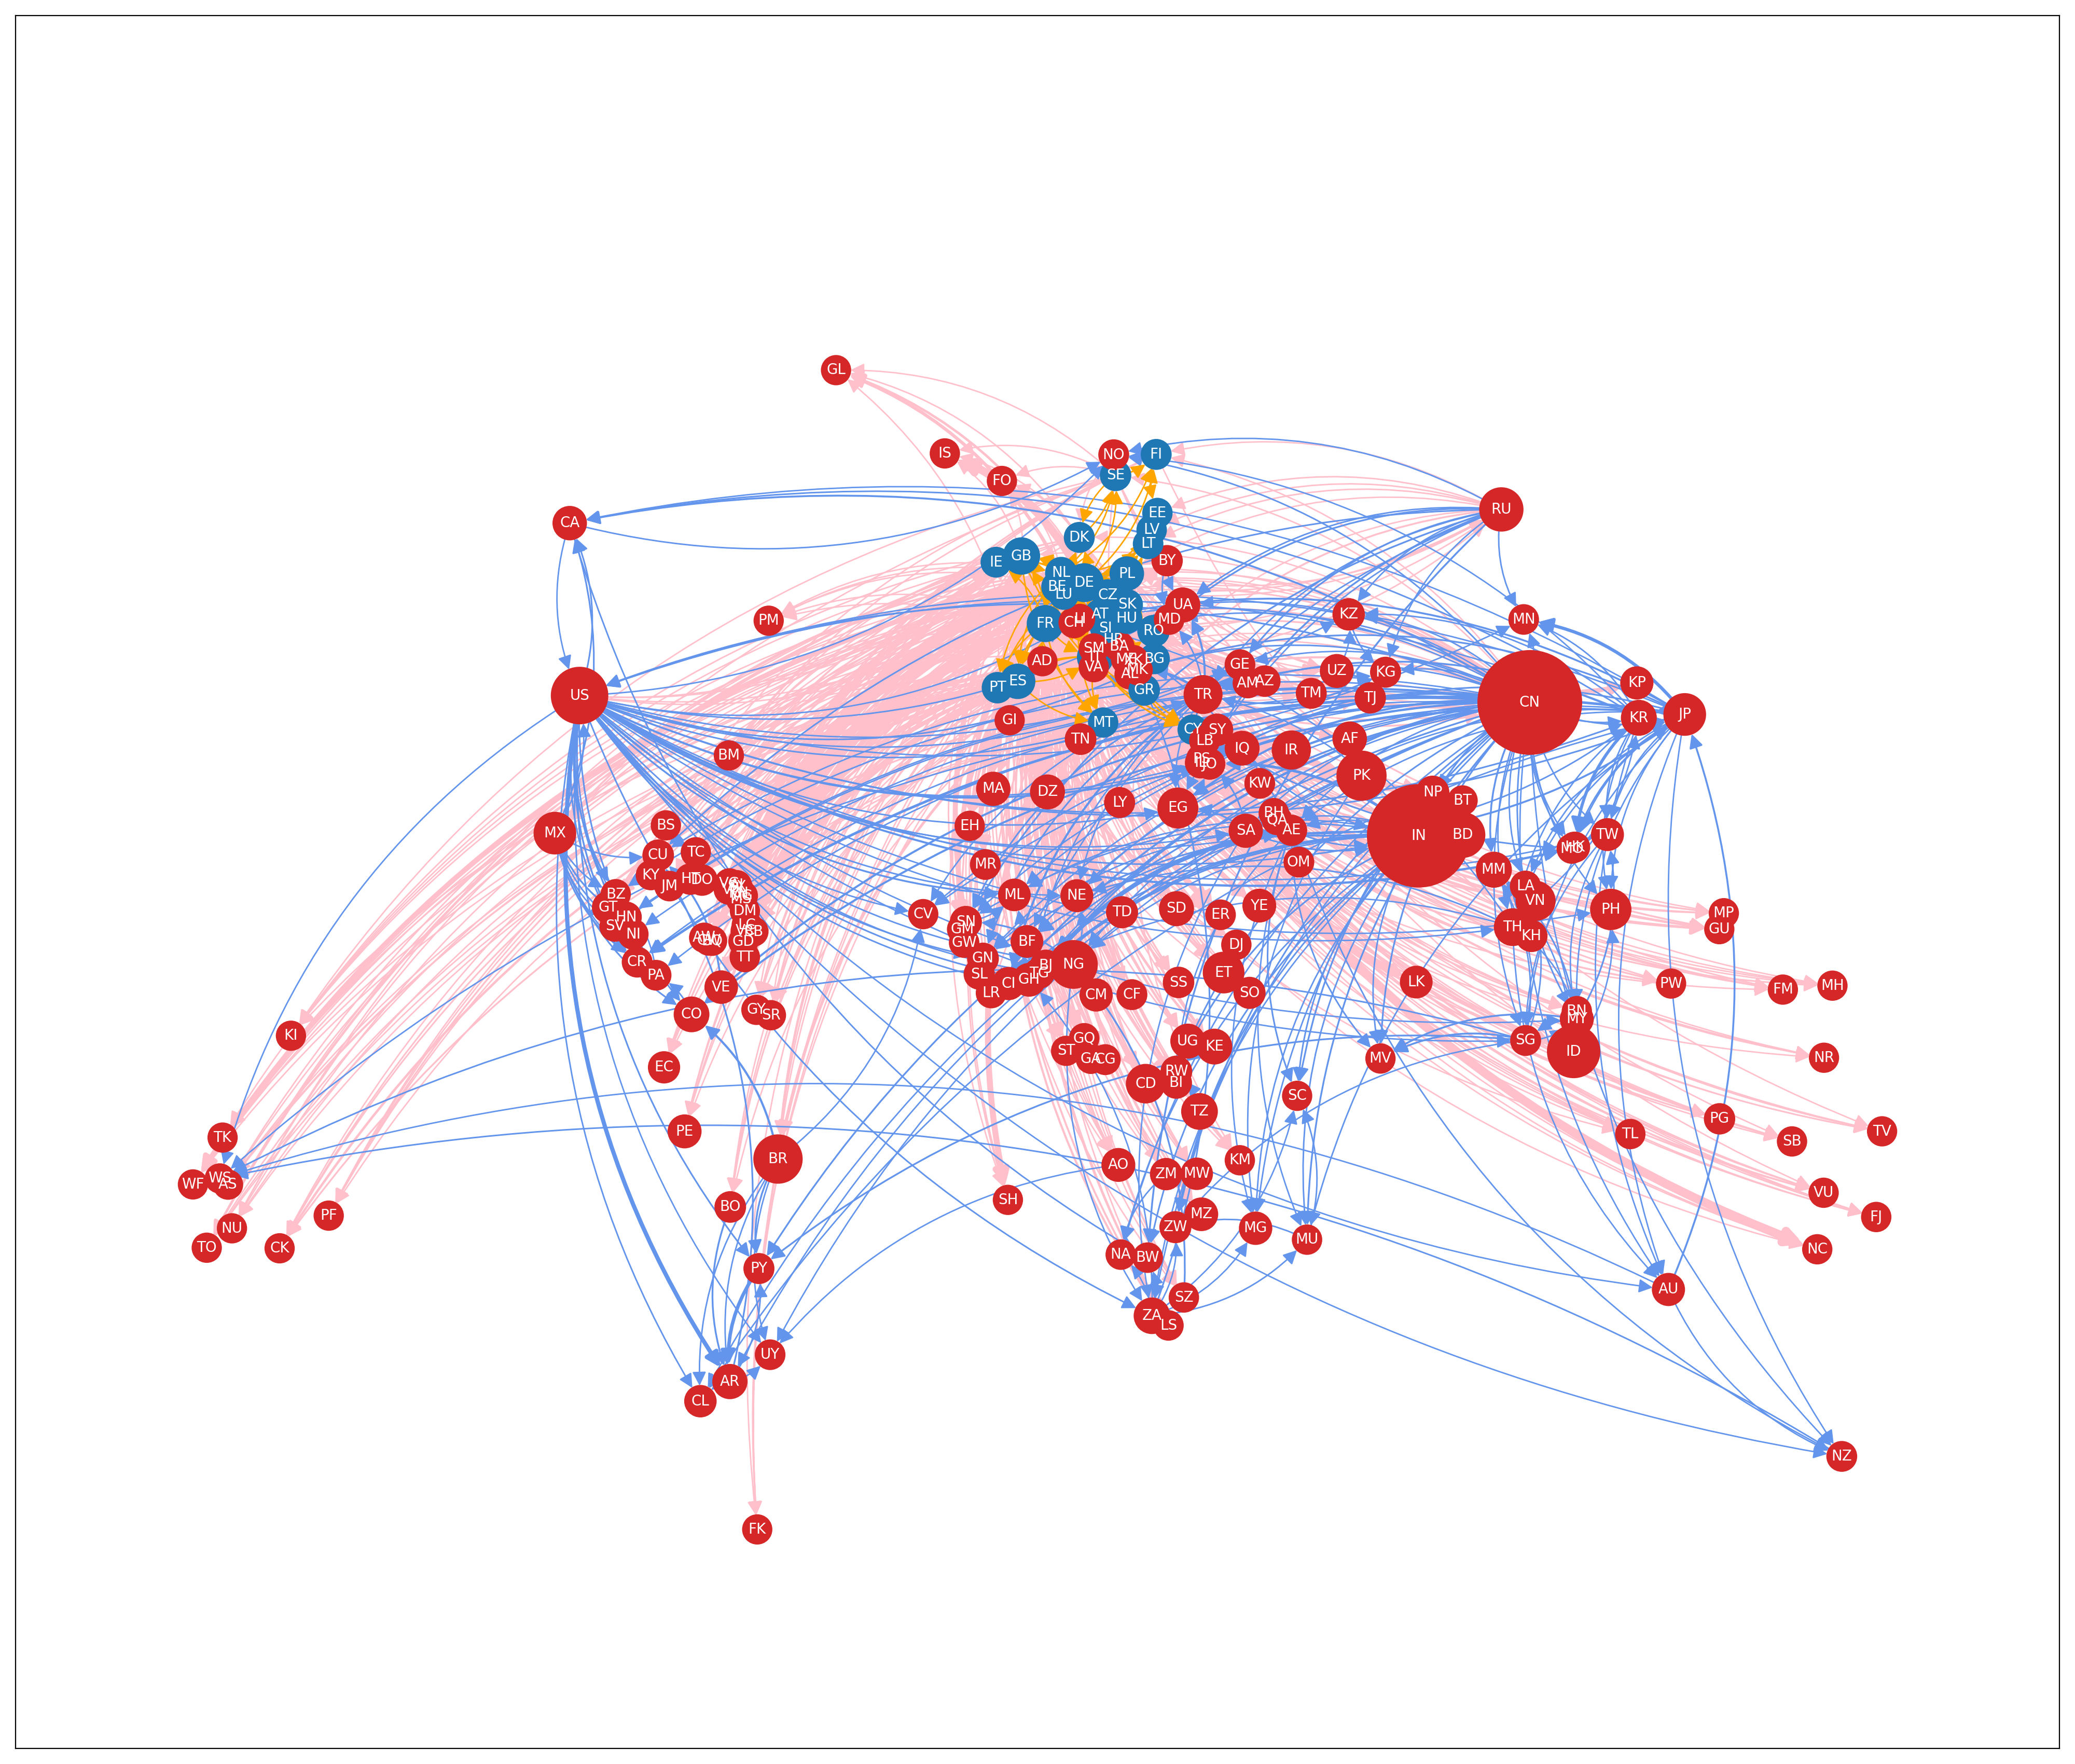
\includegraphics[width=\textwidth]{pics/full_y19_pTO_geo.png}
    \caption[Global trade network of all products in 2019.]{Global trade network of all products in 2019. Nodes are positioned according to the geographical location of the country, and their size is proportional to the population. The color of the node indicates EU countries (\textit{blue}) and non-EU (\textit{red}); the color of the edge is \textit{orange} for intra-EU exchanges, \textit{pink} for EU - non-EU exchanges and \textit{azure} for extra-EU exchanges. Only the top 5 import partnership for each country are shown.}
    \label{fig:geograph}
\end{figure}
What we can see in this plot is the complex net of trade routes among countries all around the world, and it emerges the important role that the greatest economies such as the US and China play in the global scenario. On the contrary, since all the blue nodes belonging to the European Union are so close to each other, it is impossible to see the web of intra-EU exchanges. What \textcite{benedictis2014bacicepii} point out, in fact, is that this picture does not give full account of the implication of the interdependence among countries, and using geographical positions we can draw conclusions only about the bilateral trades of countries, not their ensemble. In their words, ``\textit{this is the visual analog of the assumption of conditional independence among dyads imposed on international trade flows}".
If we want countries' interactions to be accounted in determining the relative position of each nation in the whole trading network, we should ignore their geographical position and move from a physical space to a \textit{topological space}. In the following part, we will employ Network Analysis methods to carry out this goal and improve the visualization of the graph.

\subsection{Force-Directed Algorithms}
Instead of using the geographical position of the countries, we can apply what is called a \textit{force-directed} algorithm to plot the nodes of the graph. In brief, this kind of algorithms act as a balanced spring system that minimizes the energy in the system: it is as if countries were linked through springs. Countries which are connected with an edge tend to stay close (as if there were a force that attracts them), while countries which are not connected tend to be placed far apart. In doing so, the position of each country does not depend only on its links but also on the indirect effect of its neighbors' neighbors: this is to say that countries are not affected just by their trade partners but also by entire groups or clusters of countries. In particular, the technique that we apply here is the one proposed by \textcite{fruchterman1991graph}.
The main consequence of this method is that we can now interpret the position of nodes relatively to all the other countries in the trade graph. This is an added benefit, since we can observe the effect of a relationship between any two trading countries and the whole structure of the network itself, showing patterns that were difficult to see in the previous visualization. An example of this can be seen in Figure \ref{fig:forcedir}, which displays the same graph as before, but with a spring layout from the force-directed algorithm.
\begin{figure}
    \centering
    \includegraphics[width=\textwidth]{pics/full_y19_pTO_force_20.png}
    \caption[Global trade network of all products in 2019.]{Global trade network of all products in 2019. Nodes are positioned according to the force-directed algorithm, and their size is proportional to the population. The color of the node indicates EU countries (\textit{blue}) and non-EU (\textit{red}); the color of the edge is \textit{orange} for intra-EU exchanges, \textit{pink} for EU - non-EU exchanges and \textit{azure} for extra-EU exchanges. Only the top 5 import partnership for each country are shown.}
    \label{fig:forcedir}
\end{figure}
By construction, each node has only 5 incoming links, which is equivalent to say that their in-degree is 5. The weights of these edges change depending on the strength of the partnership, which in our case is measured in average expense for 1000 inhabitants. If on the one hand the in-degree is fixed, we cannot say the same in advance for the out-degree, and it is this difference across countries which plays a key role in the visualization layout. Highly connected nodes are generally placed at the center of the network, while countries which are less connected are placed near the borders of the figure. For a node to have many links means that a lot of countries have it in their top-5 list of importing partners. In the figure, we can spot these nodes easily, since they are the most central ones, such as China (CN), the United States (US) and Germany (DE). We see that a lot of links origin from these nodes and go towards both near and peripheral countries, and in fact, being tied to many nodes is the reason why the layout has put them in a central position. A network with this structure is called \textit{core-periphery}. In general, this structure consists of a core cluster which is internally cohesive, and one or more other positions with ties to the core cluster, but not to each other. These peripheral positions may or may not be internally cohesive \cite{wasserman1994social}. This resembles the network in Figure \ref{fig:forcedir}, where all the countries which are at the periphery of the graph are linked with the more important economies at the center, while this center countries have a high level of connections among them.
A second thing that we can observe by comparing the two plots is the impact of \textit{pink} edges, i.e. exchanges between one EU and one non-EU country. While in the first plot we see that the European Union has a great number of exchanges with south-American countries and Pacific islands, this web does not appear more important than the \textit{azure} links (among extra-EU). When we move instead to the second visualization, the comparison is much more evident: the ratio of pink edges against azure ones breaks in favor of the former and it is easier to see that a high number of peripheral nations trade considerably with the EU. In fact, the number of pink edges in this specific case is 699, while the number of azure ones is 320. 
A final relevant information is conveyed by the size of the nodes: since we use population as the normalizing constant for the weight of the edges, in both plots a bigger node represents a more populous country. Showing it in the visualization allows us to compare more easily countries with similar size. For example, we can compare China (CN) and India (IN), the two biggest nations in terms of inhabitants, and we immediately see that in terms of exports China has a more central role in the world network than India: in fact, the out-degree of China is 78 while that of India is 22.\\
Given all the reasons that are explained in this paragraph, it is easy to see that the kind of layouts using force-directed algorithms are much more informative than the ones on the geographical space. Hence, from here onward, all graphs will be plotted in this way.


%\pagebreak
\section{PageRank, Hubs and Authorities}\label{sec:4pagerank}

In the world trade network, most countries are characterized by weak trade links, but there exists a group of advanced countries featuring a large number of strong relationships \cite{deguchi2014hubs}, which suggests a core-periphery structure \cite{fagiolo2010evolution}. As pointed out before, we can have an understanding of the network by looking at the centrality measures of its nodes (in- and out-degree) or of the entire graph (average degree, density). However, node degrees are computed using only local information, since for every node it is enough to know the connections with its neighbors. Let me introduce now a centrality measure that instead takes into account the relationships of the entire network and their effect on the node under consideration: the PageRank. 
First introduced by \textcite{page1999pagerank}, this measure of centrality of a node is influenced by the same measure for the neighboring nodes, and it is proportional to their PageRank divided by their out-degree. What this means is that nodes which point to many others give only a small amount of centrality on to each of those others, even if their own centrality is high. Hence, to compute a node's PageRank we need to know its neighbors' PageRank, and so on, showing the fact that the information for each single node comes from the whole graph. Intuitively, we can think of PageRank as a kind of ``fluid" that circulates through the network, passing from node to node across edges following their direction, and accumulating at the nodes which are most important \cite{easley2012networks}. To be more precise, we compute PageRank ($pr$) in the following way:
\begin{enumerate}
    \item Given a graph with $n$ nodes, we start by assigning to all nodes the same initial value for $pr$, set to $1/n$;
    \item Choose a number $k$ of iterations, and for $k$ steps repeat:\\
            Each node divides its current $pr$ equally across its out-going links, and passes these equal shares to the pages it points to. Each node updates its new $pr$ as the sum of the shares that it receives from the neighbors.
\end{enumerate}
One can prove that (except in certain degenerate cases) the PageRank values of all nodes converge to limiting values as the number of steps $k$ goes to infinity. To avoid cases in which the total available $pr$ in the network ends up in nodes that have no link that can give it back, we can introduce a \textit{scaled} version of the PageRank, whose formula is
\begin{equation}\label{eq:pagerank}
    pr_i = \alpha \sum_{j} a_{ij} \frac{pr_j}{k_j^{out}} + \beta
\end{equation}
where $\alpha$ and $\beta$ are positive constants, $a_{ij}$ is an entry of the adjacency matrix and $pr_i$ and $pr_j$ are the PageRank values of nodes $i$ and $j$, respectively. 
The economic significance of this centrality measure is that a country with high PageRank centrality is connected to a central country, which is also a country with high PageRank centrality, indicating that they are core sources in that specific market.
An alternative way to define the PageRank of a graph is the eigenvector of the following Google matrix:
\begin{equation}\label{eq:googlemat}
    g_{ij} = q \frac{a_{ij}}{\sum a_{ij}} + (1-q)\frac{1}{N}
\end{equation}
Here $q = 0.85$ is a positive parameter introduced to ensure the existence of a unique solution. If we denote by $\mathbf{G}$ the Google matrix defined above, then we can obtain the vector of PageRank values $\mathbf{z} = (z_1,\dots,z_N)^T$ by repeating the following iteration until convergence:
\begin{equation}
    \mathbf{z(t+1) = G^T z(t)}
\end{equation}
In recent years, a major topic in network science research has been the investigation of the effects of ranking algorithms on the performance and behavior of networked systems. \textcite{ermann2011google} found that the page rank approach gives a ranking that is independent of the trade amount of a given country.
PageRank centrality assigns high centrality values to those nodes which have a high number of incoming edges from other nodes with high centrality. In terms of countries and trade, a country has high PageRank if it imports from other countries with high PageRank. Countries instead which have a high number of outgoing links with a large amount of trade, and hence have low values of PageRank, are called \textit{hubs}. In the next paragraph I will show how to find countries which are hubs and their interpretation.

\paragraph{Hubs and Authorities}
According to what is reported by \textcite{deguchi2014hubs}, an economic \textit{hub} country usually imports raw materials, parts, and intermediate goods from other countries, assembles final goods and exports these goods to other countries. % Maybe talk about China being a hub country, if verified
Therefore, differently from the PageRank importance, we can also define a node's centrality based on whether it \textit{points to} other countries with high importance, which in our case is a country that exports to other central countries \cite{sajedianfard2021quantitative}. On the other hand, we could define the importance of a node based on whether it is \textit{pointed at} by many others. Following this line, we could differentiate the types of central countries that we can find in networks, and we call them:
\begin{itemize}
    \item \textbf{\textit{Hubs}}: The countries that trade with important and central points (with respect to that specific trade market) and they export to other important and central countries (the authorities) of the network;
    \item \textbf{\textit{Authorities}} The countries that are important and central points of a specific trade market in the import sector.
\end{itemize}
To put it simply, a node with a high authority value is pointed to by many other nodes with high hub values, and a node with a high hub value points to many nodes with high authority values. Note however that an authority may also be a hub and vice versa. In the context of the world trade network, authorities are countries that receive a lot of imports, from many countries, and thus are dependent from them for that specific product. Contrary to what the name suggests, very often countries with high authority values are small countries that completely depend on imports from others for their demand of goods. Instead, hubs are countries that are typically producers or manufacturers of goods and that export those goods to a high number of other countries.
To compute the hub and authority values of the nodes in the network, I use an algorithm called Hyperlink-Induced Topic Search (HITS), which was originally introduced by \textcite{kleinberg1999authoritative}. Let me define the vector of HITS authority values as $\mathbf{x}=(x_1,\cdots,x_N)^T$, and the vector of HITS hubs as $\mathbf{y}=(y_1,\cdots,y_N)^T$. Similarly to the $pr$ values, the two metrics are defined by the limit of the following set of iterations:
\begin{align}\label{eq:hits}
    \mathbf{x}^{t+1} &= c(t) \mathbf{A}^T \mathbf{y}^t \\
    \mathbf{y}^{t+1} &= d(t) \mathbf{A} \mathbf{x}^{t+1} 
\end{align}
where $c(t)$ and $d(t)$ are normalization factors to force the sums of all elements equal to one, as we impose that for every $t$
\begin{align*}
    \sum_{i=1}^N x_i^{t} = 1 \\
    \sum_{i=1}^N y_i^{t} = 1 \,.
\end{align*}
The initial values of the iterations are $x_i = 1/N$ and $y_i = 1/N$ for all nodes $i$. What can be seen from Equation \ref{eq:hits} is that the HITS authority vector $\mathbf{x}$ is the eigenvector of the matrix $\mathbf{A^T A}$, while the HITS hub vector $\mathbf{y}$ is the eigenvector of $\mathbf{A A^T}$ \cite{deguchi2014hubs}.

\section{Community detection}\label{sec:4community}
A fundamental modern technique in the analysis of network data is the automatic discovery of communities, which are groups of nodes that are strongly connected or that share similar features or roles. However, community detection is a rich and challenging problem since there is no clear definition on what constitutes a community: usually, communities are defined as non-overlapping groups of nodes such that there are more edges within groups than between them, but this definition doesn't cover all cases and leaves space to many computationally approaches to detect them \cite{fortunato202220years}. In the next sections, I will overview two of the most common approaches: the \textit{Louvain method} and the \textit{Stochastic Block Model}. 
The first approach is based on an optimization problem: we have a function that, given a division of the network in communities, returns a score such that a ``good" division gets a higher score, and our goal is to maximize it. The most common score is the quality function known as modularity, which explicitly favors divisions with many edges within groups.
The second approach instead is based on statistical inference, where we assume that communities are not just a feature of the network structure, but a primary driver of it. Nodes are connected precisely because of the community they belong to, and not the other way around. The placement of edges is represented using a probabilistic model, in which the probability that two nodes are connected depends uniquely on the communities they belong to. A ``good" community structure is one who has a high probability of generating the observed network through the model, so that we can use this probability as a score function.
These are the two approaches for community detection that I will apply to the world trade networks, in order to see whether I can uncover any underlying structure of the trade relationships that is not apparent from a qualitative view of the graph or through the other metrics that I have described so far in the chapter.

\subsection{Louvain method}

The Louvain Community Detection algorithm, or Louvain method, is a simple optimization method to extract the community structure of a network. It is a heuristic method whose goal is to maximize the \textit{modularity} function. The modularity of a network is a measure of the structure of the graph, which quantifies the strength of the division of the nodes into modules (i.e. communities). In general, networks with high modularity have dense connections between the nodes within a community but sparse connections between nodes in different communities.
For weighted directed networks, the formulation of modularity is 
\[
    Q = \frac{1}{m} \sum_{ij} \left[ W_{ij} - \frac{k_i^{in}k_j^{out}}{m} \right] \delta(c_i,c_j)
\]
where $W_{ij}$ is the weight of the edge $(i,j)$, $k^{in}$ and $k^{out}$
are the in-degree and out-degree of nodes, $c_i$ indicates the community of node i and the $\delta$-function $\delta(c_i,c_j)$ is equal to 1 if $c_i=c_j$ or $0$ otherwise \cite{leicht2008community}.
Therefore, we use Louvain algorithm to find the configuration of communities that maximizes modularity. Starting from a weighted directed network of $N$ nodes, the method works in two phases. 
In the first phase, we start by assigning a different community to each node of the graph, thus starting with as many communities as nodes. Then for each node $i$ we consider the neighbors $j$ of $i$ and we evaluate the gain in modularity that would take place by removing $i$ from its community and adding it to the community of $j$. Then, node $i$ is placed in the community such that we have the greatest positive gain possible in modularity, otherwise $i$ stays in the original community if there is no improvement \cite{blondel2008louvain}. We can directly compute the modularity gain $\Delta Q$ obtained by moving an isolated node \(i\) into a community \(C\) as
\[
    \Delta Q = \frac{k_{i,in}}{m} - \gamma\frac{k_i^{out} \cdot\Sigma_{tot}^{in} + k_i^{in} \cdot \Sigma_{tot}^{out}}{m^2}
\]
where \(k_i^{out}\), \(k_i^{in}\) are the outer and inner weighted degrees of node \(i\) and \(\Sigma_{tot}^{in}\), \(\Sigma_{tot}^{out}\) are the sum of in-going and out-going links incident to nodes in \(C\).
The parameter $\gamma$ is called \textit{resolution}, and its function is to assign a preference to larger (when $\gamma < 1$) or smaller (when $\gamma > 1$) communities \cite{hagberg2008networkx}.
This process is repeated sequentially for all nodes until we have no more improvement available and the first phase is complete.
The second phase then consists in creating an auxiliary network whose nodes are now the communities found during the first phase. The weights of the edges between the new nodes are given the sum of the weight of the edges between nodes in the corresponding two communities (links between nodes of the same community lead to self-loops in the new network). Once the network is constructed, we can reapply the first phase and construct new communities. Denoting by \textit{pass} each two-phase step of the optimization, we note that by construction the number of communities decreases at each pass. We iterate each pass until there are no more changes that induce a gain in modularity, and this means we have reached a maximum \cite{blondel2008louvain}.


%\pagebreak
\subsection{Stochastic Block Model}\label{sec:sbm}
Stochastic block models (SBM) are an increasingly popular class of models in the field of statistical analysis of graphs and networks. They can be used to discover or understand the latent structure of a network, as well as for clustering purposes. In our particular case, I will apply this method on the trade graphs to discover if any communities or clusters emerge and find an interpretation for them.
I will proceed now to describe a formal version of the stochastic block model, together with the needed terminology. This part is adapted from \textcite{lee2019review}.\\
Let us consider a graph $\mathcal{G} = (\mathcal{N},\mathcal{E})$, where $\mathcal{N}$ is the node set of size $N = |\mathcal{N}|$, and $\mathcal{E}$ is the edge set of size $M = |\mathcal{E}|$. Taking two nodes $p$ and $q$ from $\mathcal{N}$, we call a pair of nodes a \textit{dyad}, and the existence of an edge for the dyad $(p,q)$ is denoted by $\mathbf{A}_{pq}$ which is an element of the $N \times N$ adjacency matrix $\mathbf{A}$. Recall that if $\mathcal{G}$ is directed, as in our case, then the adjacency matrix is not symmetric and $\mathbf{A}_{pq}$ is independent of $\mathbf{A}_{qp}$.
In the SBM, each node belongs to one of the $K$ groups (which are less than $N$): since the groups are unknown before modeling, for nodes $p = 1,\ldots,N$ we also define a vector $\mathbf{Z}_p$ of dimension $K$ which is a one-hot vector representing the membership of node $p$. This means that all the elements of $\mathbf{Z}_{p}$ are $0$ except for one position, call it $k$, which is equal to $1$, signifying that node $p$ belongs to group $k$.
Similar to $\mathbf{Z}_{p}$, we also define a $N \times K$ matrix $\mathbf{Z}$ as
\[
    \mathbf{Z} = (\mathbf{Z}_1 \cdots \mathbf{Z}_n)^T
\]
where we call $\mathbf{Z}_{pi}$ the $i$-th element of $\mathbf{Z}_p$.\\
If we take $\mathbf{Z}$ and we sum over the rows, then we can obtain a vector $\mathbf{N} = (N_1 \cdots N_K)^T$ of the group sizes, since the vectors $\mathbf{Z}_{p}$ are zero-one.
In order to describe the generation of the edges of $\mathcal{G}$ according to the group the nodes belong to, we introduce a $K \times K$ block matrix $\mathbf{C}$. Given that $\mathcal{G}$ is directed, we have that for every community $1 \leq i,j \leq K$, $\mathbf{C}_{ij}$ represents the probability of having a directed edge from a node in $i$ to a node in $j$. The idea of the block matrix $\mathbf{C}$ is that the dyads are conditionally independent given the group memberships $\mathbf{Z}$. Equivalently, we could also say that
\[
    \mathbf{A}_{pq} \sim Bernoulli(\mathbf{Z}^T_p \mathbf{C} \mathbf{Z}_q),
\]
that is to say that $\mathbf{A}_{pq}$ follows a Bernoulli distribution where the success probability is the probability of having a node between the two groups to which $p$ and $q$ belong to. Furthermore, $\mathbf{A}_{pq}$ is independent of $\mathbf{A}_{rs}$ for $(p,q) \neq (r,s)$, given $\mathbf{Z}_p$ and $\mathbf{Z}_q$.\\
The assumption that the edge probability of a dyad depends only on their memberships is based on the concept of \textit{stochastic equivalence}: for nodes $p$ and $q$ in the same group, the probability of $p$ connecting with node $r$ is equal and independent to the probability of $q$ connected with $r$. This concept does not require that the nodes in the same group are more connected within themselves than with nodes in another group, but essentially it means that they express the same characteristics in terms of which nodes (of which group) they are connected to. We can also say this by noting that the elements among the major diagonal of $\mathbf{C}$ are not necessarily higher than the off-diagonal elements.\\
Given $\mathbf{Z}$ and $\mathbf{C}$, and given the assumption that the edges are Bernoulli distributed conditional on the group memberships, then we can write down the likelihood as 
\begin{equation}\label{eq:sbmlik}
    \pi (\mathbf{A}|\mathbf{Z},\mathbf{C}) = \prod_{p\neq q}^n \pi(\mathbf{A}_{pq}|\mathbf{Z},\mathbf{c}) 
    = \prod_{p\neq q}^n \left[ \left( \mathbf{Z}^T_p \mathbf{C} \mathbf{Z}_q \right)^{\mathbf{A}_{pq}} \left( 1 - \mathbf{Z}^T_p \mathbf{C} \mathbf{Z}_q \right)^{(1-\mathbf{A}_{pq})} \right]
\end{equation}
By applying a change of index, we can rewrite \ref{eq:sbmlik} as
\begin{equation}
    \pi (\mathbf{A}|\mathbf{Z},\mathbf{C}) = \prod_{i \leq j} \mathbf{C}^{\mathbf{E}_{ij}}_{ij} (1 - \mathbf{C}_{ij})^{(\mathbf{N}_{ij} - \mathbf{E}_{ij})}
\end{equation}
where we have that $\mathbf{E}$ is a $K \times K$ adjacency matrix between groups, i.e. $E_{ij}$ is the number of edges going from block $i$ to block $j$ in the case of directed graphs. We also have $\mathbf{N}_{ij} = \mathbf{N}_i\mathbf{N}_j$ if $i \neq j$, $\mathbf{N}_{ij} = \mathbf{N}_i(\mathbf{N}_i-1)$ if $i=j$.\\
When applying SBMs to real-world data, such as in our case, usually neither $\mathbf{Z}$ nor $\mathbf{C}$ is known, and they have to be inferred, therefore we need to make assumption before modelling. For $p = 1,...,n$, we assume that the latent variable $\mathbf{Z}_p$ is independent of $\mathbf{Z}_q$ a priori. We also assume that $P(\mathbf{Z}_{pi}=1) = \theta_i$, where $\theta_i$ is the $i$-th element of the $K$-vector $\mathbf{\theta} = (\theta_1 \dots \theta_K)^T$ such that $\sum_{i=1}^K \theta_i = 1$. Essentially, we could say that the latent group $\mathbf{Z}_p$ follows the multinomial distribution with probabilities $\mathbf{\theta}$, that is
\begin{equation}
    \pi(\mathbf{Z}|\theta) = \prod_{p=1}^n \mathbf{Z}_p^T \theta = \prod_{p=1}^n \theta^T \mathbf{Z}_p = \prod_{i=1}^K \theta^{N_i}_i
\end{equation}

\subsubsection{Degree-Corrected SBM}
A variant of the previously shown SBM is the Degree Corrected SBM, proposed by \textcite{karrer2011dcsbm}. Here the authors are working with multigraphs, and they propose to redefine $\mathbf{A}_{pq}$ to be the number of edges for the dyad $(p,q)$ and they assume it follows a Poisson distribution, while $\mathbf{C}_{ij}$ is the \textit{expected} number of edges from a node in group $i$ to a node in group $j$. The density of $\mathbf{A}_{pq}$ becomes
\begin{equation}\label{eq:poisSBMdens}
    \pi(\mathbf{A}_{pq}|\mathbf{Z,C}) = (\mathbf{A}_{pq}!)^{-1} \exp \left( -\mathbf{Z}^T_p \mathbf{C} \mathbf{Z}_q \right) \left( \mathbf{Z}^T_p \mathbf{C} \mathbf{Z}_q \right)^{\mathbf{A}_{pq}}
\end{equation}
What they claim is that in the limit of a large sparse graph, the edge probability equals the expected number of edges, therefore this version of the SBM (called Poisson SBM) is asymptotically equivalent to the Bernoulli counterpart, presented above.\\
Their proposal, however, doesn't stop here, since so far we have just changed the likelihood of the model. What they introduce is a new parameter $\phi_p$ for each node $p$: the $\phi$'s are subject to the constraint that $\sum_{p=1}^N \phi_p \mathbb{1}\{\mathbf{Z}_{pi} = 1\} = 1$ for every group $i$, so that the expected number of edges for the dyad $(p,q)$ is now $\phi_p \phi_q \mathbf{Z}^T_p \mathbf{C} \mathbf{Z}_q$. Thus, the density of $Y_{pq}$ in \ref{eq:poisSBMdens} becomes
\begin{equation}\label{eq:dcsbm}
    \pi(\mathbf{A}_{pq}|\mathbf{Z,C,\phi}) = (\mathbf{A}_{pq}!)^{-1} \exp \left( -\phi_p \phi_q \mathbf{Z}^T_p \mathbf{C} \mathbf{Z}_q \right) \left(\phi_p \phi_q \mathbf{Z}^T_p \mathbf{C} \mathbf{Z}_q \right)^{\mathbf{A}_{pq}}
\end{equation}
where $\mathbf{\phi} = (\phi_1 \cdots \phi_N)^T$.\\
Equation \ref{eq:dcsbm} is what is called the Degree-Corrected (DC) SBM. We can interpret the parameters $\phi_p$ and $\mathbf{C}_{ij}$ as their maximum likelihood estimates: $\phi_p$ can be seen as the ratio of the degree of $p$ to the sum of the degrees in $p$'s block, while $\mathbf{C}_{ij}$ as the total number of edges between groups $i$ and $j$ \cite{lee2019review}.
% As in the Bernoulli version, also here we can rewrite the likelihood based on the equation above by making a change of indices from nodes $p,q$ to blocks $i,j$ as
% \begin{equation}
%     \pi(\mathbf{A}|\mathbf{Z,C,\phi}) = \prod_{p<q}^N (\mathbf{A}_{pq}!)^{-1} \exp \left( -\phi_p \phi_q \mathbf{Z}^T_p \mathbf{C} \mathbf{Z}_q \right) \left(\phi_p \phi_q \mathbf{Z}^T_p \mathbf{C} \mathbf{Z}_q \right)^{\mathbf{A}_{pq}}
% \end{equation}
What \textcite{karrer2011dcsbm} argue in their paper for DCSBM is that the simple block model doesn't work well in many applications to real world networks, and in particular, it is not flexible enough to generate graphs with structure similar to that found in empirical data. This means that community detection, seen here as \textit{a posteriori} fit of the model to the data, gives poor results, since in fact in the original SBM the expected degree is the same for all nodes in each group. The simple variation that they introduce is to include heterogeneity in the degrees of vertices, and they show that in this way they are able to improve the performance of the models for statistical inference of group structure.


% Analysis chapter
\chapter{Methods and Analysis chapter}

% Take my thesis and copy the style, however, basically what you did and how you did it 
% So 
% \begin{itemize}
%     \item Each method \& analysis has its section
%     \item Draw some conclusions about this (here \textbf{technical} ones!)
% \end{itemize}


% Conclusions
\chapter{Conclusions}\label{ch:5conclusions}

After terminating the empirical analysis of two sectors in the world trade network, let me proceed by recalling what was the goal of this research thesis and how the proposed work aligns with that.
Given the datasets that I started with, the purpose was to extract from them a suitable set of structured data to easily support the construction of the trade networks. I had to overcome some difficulties and to adapt the nomenclatures and currencies in order to properly merge the information from Eurostat and from WTO. Once I achieved this intermediate step, the next task was to explore the vast literature of Social Network Theory and to choose the most appropriate techniques for studying this kind of weighted directed graphs, in which not all graph theory concepts (such as the path between two nodes) could find an interpretation and be applied. The statistical techniques that I evaluated can be summarized as a group of graph and node properties, measured through properly defined metrics which highlight different aspects of the network structure, and then the two algorithms (Stochastic Block Model and Louvain Method) that I overviewed and applied for the task of community detection. Finally, once the structured normalized dataset was built, and the statistical methods were studied, I wanted to combine the two and apply the reviewed techniques to some real-life scenarios like the world trade sectors of \textit{Food Products} and \textit{Crude petroleum and natural gas}. What I found out in the end is that, taken one by one, the methods of network analysis may have some shortcomings in capturing the full picture, but if instead they are analyzed together with the available metrics and algorithm output, they are quite powerful in providing us with an insightful and newer understanding of the global patterns in international trade.
Therefore, we can conclude that given a dataset of historical records of bilateral trade relations among countries, it is possible to build a methodology to begin studying the data using a tool set of descriptive statistics and network science methods. Such a step is of paramount importance in whatever statistical analysis one wants to conduct on a similar dataset, which can be either for modelling purposes or for the forecasting of policies and scenarios. 
However, such statistical procedures have their limitations: for example, when presented with two different methods for the same task, as in the case of community detection, one needs to be able to discern which parameter setting and which outcome is best representing the patterns and dynamics of the network. In order to do so, the researcher often needs to integrate the insights from the model with his knowledge from other sources, such as a domain knowledge of the renowned relationships or monopolistic roles that are present in the world trade network.
Building upon this research, one may also want to take a step further and think about possible developments of the methodology to account for more complex layers of interactions in the networks. For example, one could study in deep the temporal component that is present in these datasets, and understand how the sequence of graphs behaves when evolving through time: this is the branch of research which deals with dynamic network and their analysis. In alternative, one could try to expand on the other relevant dimension of this dataset after time, that is the sector categories: it is possible in fact to construct multi-layer networks, in which a couple of nodes can be joined by more than one edge, in this case for example, they would be representing the groups of trade products that are exchanged, or perhaps the different means of transport that countries use to trade goods and services.

% RECAP THE GOAL
% ANSWER THE RESEARCH QUESTIONS
%   RECAP STEP TESI
% RESULTS USEFUL
% LIMITATION & DEVELOPMENTS
    % dynamic networks
    % multi-layer networks



\begin{singlespace}
% \bibliographystyle{alpha}
\printbibliography

\appendix
\chapter{Tables}

\pagebreak
\section{Nomenclatures}

\begin{tabular}{l|c}%
    \bfseries Code & \bfseries Description% specify table head
    % \csvreader[head to column names]{cpa21_l2.csv}{}% use head of csv as column names
    % {\\\hline\Code & \Description}% specify your coloumns here
\end{tabular}

\pagebreak
% \section{ISO Country Codes}
% \resizebox{1.0\textwidth}{!}
{\tiny%\tabcolsep=3pt
\begin{longtable}{lp{5cm}||lp{5cm}}
\caption{Conversion table of country names from ISO 2 codes.\label{tab:iso2}}

\toprule
ISO 2 CODE & COUNTRY NAME & ISO 2 CODE & COUNTRY NAME \\
\midrule
\endfirsthead

\toprule
ISO 2 CODE & COUNTRY NAME & ISO 2 CODE & COUNTRY NAME \\
\midrule
\endhead
\midrule
\multicolumn{4}{r}{{Continued on next page}} \\
\midrule
\endfoot

\bottomrule
\endlastfoot
 AD & Andorra & MG & Madagascar \\
 AE & United Arab Emirates & MH & Marshall Islands \\
 AF & Afghanistan & MK & North Macedonia \\
 AG & Antigua and Barbuda & ML & Mali \\
 AI & Anguilla & MM & Myanmar \\
 AL & Albania & MN & Mongolia \\
 AM & Armenia & MO & Macao \\
 AN & NL Antilles & MP & Northern Mariana Islands \\
 AO & Angola & MQ & Martinique \\
 AQ & Antarctica & MR & Mauritania \\
 AR & Argentina & MS & Montserrat \\
 AS & American Samoa & MT & Malta \\
 AT & Austria & MU & Mauritius \\
 AU & Australia & MV & Maldives \\
 AW & Aruba & MW & Malawi \\
 AZ & Azerbaijan & MX & Mexico \\
 BA & Bosnia-Herzegovina & MY & Malaysia \\
 BB & Barbados & MZ & Mozambique \\
 BD & Bangladesh & NA & Namibia \\
 BE & Belgium and Luxembourg & NC & New Caledonia \\
 BE & Belgium & NE & Niger \\
 BF & Burkina Faso & NF & Norfolk Islands \\
 BG & Bulgaria & NG & Nigeria \\
 BH & Bahrain & NI & Nicaragua \\
 BI & Burundi & NL & Netherlands \\
 BJ & Benin & NO & Norway \\
 BL & St. Barthélemy & NP & Nepal \\
 BM & Bermuda & NR & Nauru \\
 BN & Brunei Darussalam & NU & Niue \\
 BO & Bolivia & NZ & New Zealand \\
 BQ & Bonaire, Sint Eustatius and Saba & OM & Oman \\
 BR & Brazil & PA & Panama \\
 BS & Bahamas & PE & Peru \\
 BT & Bhutan & PF & French Polynesia \\
 BV & Bouvet Island & PG & Papua New Guinea \\
 BW & Botswana & PH & Philippines \\
 BY & Belarus & PK & Pakistan \\
 BZ & Belize & PL & Poland \\
 CA & Canada & PM & St Pierre and Miquelon \\
 CC & Coco Islands & PN & Pitcairn \\
 CD & Congo, Democratic Republic of & PS & Occupied Palestinian Territory \\
 CF & Central African Republic & PT & Portugal \\
 CG & Congo & PW & Palau \\
 CH & Switzerland & PY & Paraguay \\
 CI & Côte d'Ivoire & PZ & Panama Canal \\
 CK & Cook Islands & QA & Qatar \\
 CL & Chile & QP & High Seas \\
 CM & Cameroon & QQ & Stores and Provisions \\
 CN & China & QR & Stores and Provisions Intra \\
 CO & Colombia & QR & Stores and Provisions within the framework of Intra-EU trade \\
 CR & Costa Rica & QS & Stores and Provisions Extra \\
 CS & Czechoslovakia & QS & Stores and Provisions within the framework of trade with third countries \\
 CS & Serbia and Montenegro & QT & West Indies \\
 CU & Cuba & QU & Countries and territories not determined \\
 CV & Cape Verde & QU & Countries and territories not specified \\
 CW & Curacao & QV & Countries and territories not specified within the framework of Intra\_EU trade \\
 CX & Christmas Islands & QW & Countries and territories not specified within the framework of trade with third countries \\
 CY & Cyprus & QX & Countries and territories not specified for commercial or military reasons \\
 CZ & Czechia & QY & Secret countries Intra \\
 DD & Germany, Democratic Republic of & QY & Countries and territories not specified for commercial or military reasons in the framework of Intra\_EU trade \\
 DE & Germany & QZ & Secret countries Extra \\
 DJ & Djibouti & QZ & Countries and territories not specified for commercial or military reasons in the framework of trade with third countries \\
 DK & Denmark & RE & Reunion \\
 DM & Dominica & RO & Romania \\
 DO & Dominican Republic & RU & Russian Federation \\
 DZ & Algeria & RW & Rwanda \\
 EC & Ecuador & SA & Saudi Arabia \\
 EE & Estonia & SB & Solomon Islands \\
 EG & Egypt & SC & Seychelles \\
 EH & Ceuta and Melilla, Spanish Sahara & SD & Sudan \\
 EH & Western Sahara & SE & Sweden \\
 ER & Eritrea & SG & Singapore \\
 ES & Spain & SH & St Helena, Ascension and Tristan Da Cunha \\
 ET & Ethiopia & SI & Slovenia \\
 FI & Finland & SJ & Svalbard \\
 FJ & Fiji & SK & Slovakia \\
 FK & Falkland Islands & SL & Sierra Leone \\
 FK & Falkland Islands (Malvinas) & SM & San Marino \\
 FM & Micronesia, Federated states of & SN & Senegal \\
 FO & Faroe Islands & SO & Somalia \\
 FR & France & SR & Suriname \\
 GA & Gabon & SS & South Sudan \\
 GB & United Kingdom & ST & Sao Tome and Principe \\
 GD & Grenada & SU & Soviet Union \\
 GE & Georgia & SV & El Salvador \\
 GF & French Guiana & SX & Sint Marteen (Dutch part) \\
 GH & Ghana & SY & Syrian Arab Republic \\
 GI & Gibraltar & SZ & Swaziland \\
 GL & Greenland & TC & Turks and Caicos Islands \\
 GM & Gambia & TD & Chad \\
 GN & Guinea & TF & French Southern Territories \\
 GP & Guadeloupe & TG & Togo \\
 GQ & Equatorial Guinea & TH & Thailand \\
 GR & Greece & TJ & Tajikistan \\
 GS & South Georgia and South Sandwich Islands & TK & Tokelau \\
 GT & Guatemala & TL & Timor-Leste \\
 GU & Guam & TM & Turkmenistan \\
 GW & Guinea-Bissau & TN & Tunisia \\
 GY & Guyana & TO & Tonga \\
 HK & Hong Kong & TP & Portugese Timor \\
 HM & Heard Islands and McDonald Islands & TP & East Timor \\
 HN & Honduras & TR & Turkey \\
 HR & Croatia & TT & Trinidad and Tobago \\
 HT & Haiti & TV & Tuvalu \\
 HU & Hungary & TW & Taiwan \\
 ID & Indonesia & TZ & Tanzania, United Republic of \\
 IE & Ireland & UA & Ukraine \\
 IL & Israel & UG & Uganda \\
 IN & India & UM & United States Minor Outlying Islands \\
 IO & British Indian Ocean Territory & US & United States \\
 IQ & Iraq & UY & Uruguay \\
 IR & Iran, Islamic Republic of & UZ & Uzbekistan \\
 IS & Iceland & VA & Holy See (Vatican City State) \\
 IT & Italy & VC & St Vincent and the Grenadines \\
 JM & Jamaica & VD & North Vietnam \\
 JO & Jordan & VE & Venezuela, Bolivarian Republic of \\
 JP & Japan & VG & Virgin Islands, British \\
 KE & Kenya & VI & Virgin Islands, United States \\
 KG & Kyrgyzstan & VN & Viet Nam \\
 KG & Kyrgyz, Republic & VU & Vanuatu \\
 KH & Cambodia & WF & Wallis and Futuna \\
 KI & Kiribati & WS & Samoa \\
 KM & Comoros & XA & American Oceania \\
 KN & St Kitts and Nevis & XB & Canary Islands \\
 KP & Korea, Democratic People's Republic of & XC & Ceuta \\
 KR & Korea, Republic of & XI & United Kingdom (Northern Ireland) \\
 KW & Kuwait & XK & Kosovo \\
 KY & Cayman Islands & XL & Melilla \\
 KZ & Kazakhstan & XM & Montenegro \\
 LA & Lao People's Democratic Republic & XO & Australian Oceania \\
 LB & Lebanon & XP & West Bank and Gaza Strip \\
 LC & St Lucia & XR & Polar Regions \\
 LI & Liechtenstein & XS & Serbia \\
 LK & Sri Lanka & XU & United Kingdom (excluding Northern Ireland) \\
 LR & Liberia & XZ & New Zealand Oceania \\
 LS & Lesotho & YD & South Yemen \\
 LT & Lithuania & YE & Yemen \\
 LU & Luxembourg & YT & Mayotte \\
 LV & Latvia & YU & Yugoslavia \\
 LY & Libya & ZA & South Africa \\
 MA & Morocco & ZM & Zambia \\
 MD & Moldova & ZW & Zimbabwe \\
 MD & Moldova, Republic of & ZZ & No data, work code \\
 ME & Montenegro &  &  \\
\end{longtable}
}

\pagebreak
\section{UN Population}\label{app:unpop}
{\tiny
\begin{longtable}{rlllrrrrr}
\caption{Population according to UN estimates updated at 2022.\label{tab:unpop}}
\toprule
 ID & iso2 & iso3 & Country & 2000 & 2005 & 2010 & 2015 & 2020 \\
\midrule
\endfirsthead

\toprule
 ID & iso2 & iso3 & Country & 2000 & 2005 & 2010 & 2015 & 2020 \\
\midrule
\endhead
\midrule
\multicolumn{9}{r}{{Continued on next page}} \\
\midrule
\endfoot

\bottomrule
\endlastfoot
 4 & AF & AFG & Afghanistan & 19542.982 & 24411.191 & 28189.672 & 33753.499 & 38972.230 \\
 8 & AL & ALB & Albania & 3182.021 & 3032.634 & 2913.399 & 2882.481 & 2866.849 \\
 12 & DZ & DZA & Algeria & 30774.621 & 32956.690 & 35856.344 & 39543.154 & 43451.666 \\
 16 & AS & ASM & American Samoa & 58.230 & 57.254 & 54.849 & 51.368 & 46.189 \\
 20 & AD & AND & Andorra & 66.097 & 79.826 & 71.519 & 71.746 & 77.700 \\
 24 & AO & AGO & Angola & 16394.062 & 19450.959 & 23364.185 & 28127.721 & 33428.486 \\
 28 & AG & ATG & Antigua and Barbuda & 75.055 & 79.869 & 85.695 & 89.941 & 92.664 \\
 31 & AZ & AZE & Azerbaijan & 8190.337 & 8656.237 & 9237.202 & 9863.480 & 10284.951 \\
 32 & AR & ARG & Argentina & 37070.774 & 39070.501 & 41100.123 & 43257.065 & 45036.032 \\
 36 & AU & AUS & Australia & 19017.963 & 20171.731 & 22019.168 & 23820.236 & 25670.051 \\
 40 & AT & AUT & Austria & 8010.428 & 8227.034 & 8362.829 & 8642.421 & 8907.777 \\
 44 & BS & BHS & Bahamas & 325.014 & 347.804 & 373.272 & 392.697 & 406.471 \\
 48 & BH & BHR & Bahrain & 711.442 & 901.921 & 1213.645 & 1362.142 & 1477.469 \\
 50 & BD & BGD & Bangladesh & 129193.327 & 140912.590 & 148391.139 & 157830.000 & 167420.951 \\
 51 & AM & ARM & Armenia & 3168.523 & 3047.246 & 2946.293 & 2878.595 & 2805.608 \\
 52 & BB & BRB & Barbados & 264.657 & 269.477 & 274.711 & 278.083 & 280.693 \\
 56 & BE & BEL & Belgium & 10264.343 & 10516.978 & 10877.947 & 11248.303 & 11561.717 \\
 60 & BM & BMU & Bermuda & 61.371 & 62.959 & 63.447 & 63.144 & 64.031 \\
 64 & BT & BTN & Bhutan & 587.207 & 663.323 & 705.516 & 743.274 & 772.506 \\
 68 & BO & BOL & Bolivia (Plurinational State of) & 8592.656 & 9377.388 & 10223.270 & 11090.085 & 11936.162 \\
 70 & BA & BIH & Bosnia and Herzegovina & 4179.350 & 4094.297 & 3811.088 & 3524.324 & 3318.407 \\
 72 & BW & BWA & Botswana & 1726.985 & 1892.807 & 2091.664 & 2305.171 & 2546.402 \\
 76 & BR & BRA & Brazil & 175873.720 & 186797.334 & 196353.492 & 205188.205 & 213196.304 \\
 84 & BZ & BLZ & Belize & 240.406 & 280.375 & 322.106 & 359.871 & 394.921 \\
 90 & SB & SLB & Solomon Islands & 429.978 & 482.486 & 540.394 & 612.660 & 691.191 \\
 92 & VG & VGB & British Virgin Islands & 20.104 & 23.497 & 27.556 & 29.366 & 30.910 \\
 96 & BN & BRN & Brunei Darussalam & 333.926 & 366.717 & 396.053 & 421.437 & 441.725 \\
 100 & BG & BGR & Bulgaria & 8097.691 & 7815.221 & 7592.273 & 7309.253 & 6979.175 \\
 104 & MM & MMR & Myanmar & 45538.332 & 47724.471 & 49390.988 & 51483.949 & 53423.198 \\
 108 & BI & BDI & Burundi & 6307.659 & 7388.874 & 9126.605 & 10727.148 & 12220.227 \\
 112 & BY & BLR & Belarus & 10256.483 & 9935.163 & 9731.427 & 9700.609 & 9633.740 \\
 116 & KH & KHM & Cambodia & 12118.841 & 13246.583 & 14363.532 & 15417.523 & 16396.860 \\
 120 & CM & CMR & Cameroon & 15091.594 & 17275.171 & 19878.036 & 23012.646 & 26491.087 \\
 124 & CA & CAN & Canada & 30683.313 & 32215.916 & 33963.412 & 35732.126 & 37888.705 \\
 132 & CV & CPV & Cabo Verde & 458.251 & 492.827 & 521.212 & 552.166 & 582.640 \\
 136 & KY & CYM & Cayman Islands & 39.658 & 46.727 & 54.074 & 60.911 & 67.311 \\
 140 & CF & CAF & Central African Republic & 3759.170 & 4208.834 & 4660.067 & 4819.333 & 5343.020 \\
 144 & LK & LKA & Sri Lanka & 18776.371 & 19673.866 & 20668.557 & 21336.697 & 21715.079 \\
 148 & TD & TCD & Chad & 8259.137 & 10005.012 & 11894.727 & 14140.274 & 16644.701 \\
 152 & CL & CHL & Chile & 15351.799 & 16175.311 & 17004.162 & 17870.124 & 19300.315 \\
 156 & CN & CHN & China & 1264099.069 & 1304887.562 & 1348191.368 & 1393715.448 & 1424929.781 \\
 158 & TW & TWN & China, Taiwan Province of China & 22194.731 & 22796.306 & 23083.083 & 23512.136 & 23821.464 \\
 170 & CO & COL & Colombia & 39215.135 & 42220.940 & 44816.108 & 47119.728 & 50930.662 \\
 174 & KM & COM & Comoros & 536.758 & 592.683 & 656.024 & 730.216 & 806.166 \\
 175 & YT & MYT & Mayotte & 159.215 & 187.142 & 211.786 & 249.545 & 305.587 \\
 178 & CG & COG & Congo & 3134.030 & 3672.839 & 4437.884 & 5064.386 & 5702.174 \\
 180 & CD & COD & Democratic Republic of the Congo & 48616.317 & 56550.247 & 66391.257 & 78656.904 & 92853.164 \\
 184 & CK & COK & Cook Islands & 15.897 & 15.146 & 17.212 & 17.695 & 17.029 \\
 188 & CR & CRI & Costa Rica & 3979.193 & 4315.887 & 4622.252 & 4895.242 & 5123.105 \\
 191 & HR & HRV & Croatia & 4548.434 & 4429.681 & 4368.682 & 4254.815 & 4096.869 \\
 192 & CU & CUB & Cuba & 11105.791 & 11246.114 & 11290.417 & 11339.894 & 11300.698 \\
 196 & CY & CYP & Cyprus & 948.237 & 1037.062 & 1129.686 & 1187.280 & 1237.537 \\
 203 & CZ & CZE & Czechia & 10234.710 & 10280.113 & 10464.749 & 10523.798 & 10530.953 \\
 204 & BJ & BEN & Benin & 6998.023 & 8149.419 & 9445.710 & 10932.783 & 12643.123 \\
 208 & DK & DNK & Denmark & 5340.655 & 5436.313 & 5550.849 & 5677.796 & 5825.641 \\
 212 & DM & DMA & Dominica & 68.346 & 68.674 & 68.755 & 70.007 & 71.995 \\
 214 & DO & DOM & Dominican Republic & 8540.791 & 9164.768 & 9775.755 & 10405.832 & 10999.664 \\
 218 & EC & ECU & Ecuador & 12626.507 & 13770.012 & 14989.585 & 16195.902 & 17588.595 \\
 222 & SV & SLV & El Salvador & 5958.482 & 6037.817 & 6114.034 & 6231.066 & 6292.731 \\
 226 & GQ & GNQ & Equatorial Guinea & 684.977 & 864.726 & 1094.524 & 1346.973 & 1596.049 \\
 231 & ET & ETH & Ethiopia & 67031.867 & 77469.940 & 89237.791 & 102471.895 & 117190.911 \\
 232 & ER & ERI & Eritrea & 2392.880 & 2831.732 & 3147.727 & 3340.006 & 3555.868 \\
 233 & EE & EST & Estonia & 1396.877 & 1354.662 & 1331.535 & 1314.657 & 1329.444 \\
 234 & FO & FRO & Faroe Islands & 45.660 & 48.291 & 48.410 & 48.816 & 52.415 \\
 238 & FK & FLK & Falkland Islands (Malvinas) & 3.080 & 3.204 & 3.187 & 3.408 & 3.747 \\
 242 & FJ & FJI & Fiji & 832.509 & 874.923 & 905.169 & 917.200 & 920.422 \\
 246 & FI & FIN & Finland & 5176.209 & 5246.071 & 5363.271 & 5479.461 & 5529.468 \\
 250 & FR & FRA & France & 58665.453 & 60510.079 & 62444.567 & 63809.769 & 64480.053 \\
 254 & GF & GUF & French Guiana & 164.351 & 201.259 & 228.453 & 257.026 & 290.969 \\
 258 & PF & PYF & French Polynesia & 250.927 & 271.060 & 283.788 & 291.787 & 301.920 \\
 262 & DJ & DJI & Djibouti & 742.033 & 830.861 & 919.199 & 1006.259 & 1090.156 \\
 266 & GA & GAB & Gabon & 1272.935 & 1458.353 & 1711.105 & 2028.517 & 2292.573 \\
 268 & GE & GEO & Georgia & 4265.172 & 3961.182 & 3836.831 & 3771.132 & 3765.912 \\
 270 & GM & GMB & Gambia & 1437.539 & 1660.368 & 1937.275 & 2253.133 & 2573.995 \\
 275 & PS & PSE & State of Palestine & 3139.954 & 3541.193 & 3992.278 & 4484.614 & 5019.401 \\
 276 & DE & DEU & Germany & 81551.677 & 81212.168 & 81325.090 & 82073.226 & 83328.988 \\
 288 & GH & GHA & Ghana & 19665.502 & 22496.951 & 25574.719 & 28870.939 & 32180.401 \\
 292 & GI & GIB & Gibraltar & 27.741 & 29.155 & 31.262 & 32.520 & 32.709 \\
 296 & KI & KIR & Kiribati & 88.826 & 98.164 & 107.995 & 116.707 & 126.463 \\
 300 & GR & GRC & Greece & 11038.109 & 11113.448 & 11033.783 & 10806.641 & 10512.232 \\
 304 & GL & GRL & Greenland & 56.184 & 56.887 & 56.351 & 55.895 & 56.026 \\
 308 & GD & GRD & Grenada & 107.432 & 110.254 & 114.039 & 118.980 & 123.663 \\
 312 & GP & GLP & Guadeloupe & 424.067 & 403.233 & 403.072 & 399.089 & 395.642 \\
 316 & GU & GUM & Guam & 160.188 & 164.430 & 164.905 & 167.978 & 169.231 \\
 320 & GT & GTM & Guatemala & 11735.894 & 13132.814 & 14543.121 & 16001.107 & 17362.718 \\
 324 & GN & GIN & Guinea & 8336.967 & 9140.114 & 10270.728 & 11625.998 & 13205.153 \\
 328 & GY & GUY & Guyana & 759.051 & 759.709 & 747.932 & 755.031 & 797.202 \\
 332 & HT & HTI & Haiti & 8360.225 & 9111.900 & 9842.880 & 10563.757 & 11306.801 \\
 336 & VA & VAT & Holy See & 0.651 & 0.628 & 0.596 & 0.564 & 0.520 \\
 340 & HN & HND & Honduras & 6656.725 & 7564.613 & 8450.933 & 9294.505 & 10121.763 \\
 344 & HK & HKG & China, Hong Kong SAR & 6731.195 & 6936.874 & 7132.438 & 7399.838 & 7500.958 \\
 348 & HU & HUN & Hungary & 10202.055 & 10073.525 & 9986.825 & 9844.246 & 9750.573 \\
 352 & IS & ISL & Iceland & 281.462 & 297.029 & 318.333 & 331.060 & 366.669 \\
 356 & IN & IND & India & 1059633.675 & 1154638.713 & 1240613.620 & 1322866.505 & 1396387.127 \\
 360 & ID & IDN & Indonesia & 214072.421 & 228805.144 & 244016.173 & 259091.970 & 271857.970 \\
 364 & IR & IRN & Iran (Islamic Republic of) & 65544.383 & 70182.594 & 75373.855 & 81790.841 & 87290.193 \\
 368 & IQ & IRQ & Iraq & 24628.858 & 28698.684 & 31264.875 & 37757.813 & 42556.984 \\
 372 & IE & IRL & Ireland & 3768.950 & 4121.216 & 4524.585 & 4665.760 & 4946.119 \\
 376 & IL & ISR & Israel & 6116.958 & 6714.124 & 7328.445 & 8007.778 & 8757.489 \\
 380 & IT & ITA & Italy & 56966.397 & 58199.876 & 59822.450 & 60232.906 & 59500.579 \\
 384 & CI & CIV & Côte d'Ivoire & 16799.670 & 18970.215 & 21120.042 & 23596.741 & 26811.790 \\
 388 & JM & JAM & Jamaica & 2612.205 & 2676.863 & 2733.896 & 2794.445 & 2820.436 \\
 392 & JP & JPN & Japan & 126803.861 & 127798.373 & 128105.431 & 127250.933 & 125244.761 \\
 398 & KZ & KAZ & Kazakhstan & 15236.253 & 15656.248 & 16627.837 & 17835.909 & 18979.243 \\
 400 & JO & JOR & Jordan & 5056.174 & 5678.534 & 6931.258 & 9494.246 & 10928.721 \\
 404 & KE & KEN & Kenya & 30851.606 & 35843.010 & 41517.895 & 46851.488 & 51985.780 \\
 408 & KP & PRK & Dem. People's Republic of Korea & 23367.059 & 24100.982 & 24686.435 & 25258.015 & 25867.467 \\
 410 & KR & KOR & Republic of Korea & 46788.591 & 47889.573 & 48813.042 & 50994.401 & 51844.690 \\
 412 & XK & XKX & Kosovo (under UNSC res. 1244) & 1823.286 & 1825.050 & 1792.563 & 1759.122 & 1670.698 \\
 414 & KW & KWT & Kuwait & 1934.901 & 2235.403 & 2943.356 & 3908.743 & 4360.444 \\
 417 & KG & KGZ & Kyrgyzstan & 4935.182 & 5193.114 & 5483.774 & 5914.980 & 6424.874 \\
 418 & LA & LAO & Lao People's Democratic Republic & 5430.853 & 5852.970 & 6323.418 & 6787.419 & 7319.399 \\
 422 & LB & LBN & Lebanon & 4320.642 & 4643.044 & 4995.800 & 6398.940 & 5662.923 \\
 426 & LS & LSO & Lesotho & 1998.630 & 1977.424 & 2022.747 & 2118.521 & 2254.100 \\
 428 & LV & LVA & Latvia & 2392.530 & 2233.157 & 2101.530 & 1991.955 & 1897.052 \\
 430 & LR & LBR & Liberia & 2895.224 & 3266.318 & 4019.956 & 4612.329 & 5087.584 \\
 434 & LY & LBY & Libya & 5154.790 & 5837.986 & 6491.988 & 6192.235 & 6653.942 \\
 438 & LI & LIE & Liechtenstein & 33.026 & 34.603 & 35.926 & 37.355 & 38.756 \\
 440 & LT & LTU & Lithuania & 3599.637 & 3373.533 & 3139.019 & 2963.765 & 2820.267 \\
 442 & LU & LUX & Luxembourg & 435.628 & 464.860 & 507.070 & 569.408 & 630.399 \\
 446 & MO & MAC & China, Macao SAR & 431.896 & 488.619 & 557.297 & 615.239 & 676.283 \\
 450 & MG & MDG & Madagascar & 16216.431 & 18792.171 & 21731.053 & 24850.912 & 28225.177 \\
 454 & MW & MWI & Malawi & 11229.387 & 12755.648 & 14718.422 & 16938.942 & 19377.061 \\
 458 & MY & MYS & Malaysia & 22945.150 & 25923.536 & 28717.731 & 31068.833 & 33199.993 \\
 462 & MV & MDV & Maldives & 282.507 & 307.018 & 361.575 & 435.582 & 514.438 \\
 466 & ML & MLI & Mali & 11239.101 & 13180.551 & 15529.181 & 18112.907 & 21224.040 \\
 470 & MT & MLT & Malta & 399.212 & 410.208 & 418.755 & 456.579 & 515.358 \\
 474 & MQ & MTQ & Martinique & 432.543 & 400.370 & 392.181 & 383.515 & 370.391 \\
 478 & MR & MRT & Mauritania & 2695.003 & 3012.360 & 3419.461 & 3946.220 & 4498.604 \\
 480 & MU & MUS & Mauritius & 1215.930 & 1258.048 & 1283.330 & 1293.153 & 1297.828 \\
 484 & MX & MEX & Mexico & 97873.442 & 105442.402 & 112532.401 & 120149.897 & 125998.302 \\
 492 & MC & MCO & Monaco & 32.465 & 32.141 & 33.178 & 36.760 & 36.922 \\
 496 & MN & MNG & Mongolia & 2450.979 & 2559.255 & 2702.520 & 2964.749 & 3294.335 \\
 498 & MD & MDA & Republic of Moldova & 4251.573 & 4001.382 & 3678.186 & 3277.388 & 3084.847 \\
 499 & ME & MNE & Montenegro & 633.324 & 632.875 & 631.044 & 633.966 & 629.048 \\
 500 & MS & MSR & Montserrat & 5.138 & 4.693 & 4.938 & 5.059 & 4.500 \\
 504 & MA & MAR & Morocco & 28554.415 & 30431.902 & 32464.865 & 34680.458 & 36688.772 \\
 508 & MZ & MOZ & Mozambique & 17768.505 & 20211.114 & 23073.723 & 26843.246 & 31178.239 \\
 512 & OM & OMN & Oman & 2344.253 & 2515.192 & 2881.914 & 4191.776 & 4543.399 \\
 516 & NA & NAM & Namibia & 1819.141 & 1962.865 & 2099.271 & 2282.704 & 2489.098 \\
 520 & NR & NRU & Nauru & 10.377 & 10.318 & 10.241 & 11.185 & 12.315 \\
 524 & NP & NPL & Nepal & 24559.500 & 26285.110 & 27161.567 & 27610.325 & 29348.627 \\
 528 & NL & NLD & Netherlands & 15899.135 & 16261.831 & 16617.117 & 17041.107 & 17434.557 \\
 531 & CW & CUW & Curaçao & 141.424 & 147.263 & 159.380 & 169.572 & 189.288 \\
 533 & AW & ABW & Aruba & 89.101 & 94.483 & 100.341 & 104.257 & 106.585 \\
 534 & SX & SXM & Sint Maarten (Dutch part) & 30.489 & 31.494 & 33.034 & 40.205 & 43.621 \\
 535 & BQ & BES & Bonaire, Sint Eustatius and Saba & 13.960 & 16.724 & 20.224 & 23.164 & 26.153 \\
 540 & NC & NCL & New Caledonia & 221.537 & 242.141 & 261.426 & 283.032 & 286.403 \\
 548 & VU & VUT & Vanuatu & 192.074 & 217.632 & 245.453 & 276.438 & 311.685 \\
 554 & NZ & NZL & New Zealand & 3855.266 & 4132.781 & 4346.338 & 4590.590 & 5061.133 \\
 558 & NI & NIC & Nicaragua & 5123.222 & 5454.678 & 5855.734 & 6298.598 & 6755.895 \\
 562 & NE & NER & Niger & 11622.665 & 13855.221 & 16647.543 & 20128.124 & 24333.639 \\
 566 & NG & NGA & Nigeria & 122851.984 & 140490.722 & 160952.853 & 183995.785 & 208327.405 \\
 570 & NU & NIU & Niue & 2.074 & 1.856 & 1.812 & 1.847 & 1.942 \\
 578 & NO & NOR & Norway & 4491.202 & 4623.689 & 4889.741 & 5190.356 & 5379.839 \\
 580 & MP & MNP & Northern Mariana Islands & 80.338 & 69.025 & 54.087 & 51.514 & 49.587 \\
 583 & FM & FSM & Micronesia (Fed. States of) & 111.709 & 110.940 & 107.588 & 109.462 & 112.106 \\
 584 & MH & MHL & Marshall Islands & 54.224 & 54.337 & 53.416 & 49.410 & 43.413 \\
 585 & PW & PLW & Palau & 19.726 & 19.831 & 18.540 & 17.794 & 17.972 \\
 586 & PK & PAK & Pakistan & 154369.924 & 174372.098 & 194454.498 & 210969.298 & 227196.741 \\
 591 & PA & PAN & Panama & 3001.731 & 3305.868 & 3623.617 & 3957.099 & 4294.396 \\
 598 & PG & PNG & Papua New Guinea & 5508.297 & 6498.818 & 7583.269 & 8682.174 & 9749.640 \\
 600 & PY & PRY & Paraguay & 5123.819 & 5476.878 & 5768.613 & 6177.950 & 6618.695 \\
 604 & PE & PER & Peru & 26654.439 & 28147.267 & 29229.572 & 30711.863 & 33304.756 \\
 608 & PH & PHL & Philippines & 77958.223 & 86261.250 & 94636.700 & 103031.365 & 112190.977 \\
 616 & PL & POL & Poland & 38504.431 & 38575.911 & 38597.353 & 38553.146 & 38428.366 \\
 620 & PT & PRT & Portugal & 10300.626 & 10523.315 & 10588.401 & 10365.435 & 10298.192 \\
 624 & GW & GNB & Guinea-Bissau & 1230.849 & 1379.713 & 1567.220 & 1788.919 & 2015.828 \\
 626 & TL & TLS & Timor-Leste & 878.360 & 969.313 & 1088.486 & 1205.813 & 1299.995 \\
 630 & PR & PRI & Puerto Rico & 3827.108 & 3805.559 & 3717.922 & 3497.335 & 3271.564 \\
 634 & QA & QAT & Qatar & 645.937 & 848.710 & 1713.504 & 2414.573 & 2760.385 \\
 638 & RE & REU & Réunion & 785.424 & 833.656 & 890.130 & 922.495 & 957.822 \\
 642 & RO & ROU & Romania & 21919.876 & 21092.264 & 20335.211 & 19906.079 & 19442.038 \\
 643 & RU & RUS & Russian Federation & 146844.839 & 143800.049 & 143242.599 & 144668.389 & 145617.329 \\
 646 & RW & RWA & Rwanda & 8109.989 & 9026.299 & 10309.031 & 11642.959 & 13146.362 \\
 652 & BL & BLM & Saint Barthélemy & 7.082 & 8.044 & 8.988 & 9.643 & 10.681 \\
 654 & SH & SHN & Saint Helena & 6.024 & 5.532 & 5.321 & 5.497 & 5.420 \\
 659 & KN & KNA & Saint Kitts and Nevis & 45.461 & 46.725 & 47.403 & 47.790 & 47.642 \\
 660 & AI & AIA & Anguilla & 11.047 & 12.128 & 13.172 & 14.525 & 15.585 \\
 662 & LC & LCA & Saint Lucia & 159.500 & 165.386 & 170.935 & 175.623 & 179.237 \\
 663 & MF & MAF & Saint Martin (French part) & 29.610 & 33.452 & 36.458 & 35.020 & 32.553 \\
 666 & PM & SPM & Saint Pierre and Miquelon & 6.274 & 6.115 & 6.052 & 5.978 & 5.906 \\
 670 & VC & VCT & Saint Vincent and the Grenadines & 113.813 & 112.043 & 109.308 & 106.482 & 104.632 \\
 674 & SM & SMR & San Marino & 26.823 & 29.508 & 31.608 & 33.570 & 34.007 \\
 678 & ST & STP & Sao Tome and Principe & 143.714 & 161.680 & 182.138 & 201.124 & 218.641 \\
 682 & SA & SAU & Saudi Arabia & 21547.390 & 24397.644 & 29411.929 & 32749.848 & 35997.107 \\
 686 & SN & SEN & Senegal & 9704.287 & 10974.057 & 12530.121 & 14356.181 & 16436.120 \\
 688 & RS & SRB & Serbia & 7935.022 & 7830.944 & 7653.748 & 7519.496 & 7358.005 \\
 690 & SC & SYC & Seychelles & 80.060 & 85.883 & 92.409 & 99.240 & 105.530 \\
 694 & SL & SLE & Sierra Leone & 4584.067 & 5683.334 & 6436.698 & 7314.773 & 8233.970 \\
 702 & SG & SGP & Singapore & 4053.602 & 4344.637 & 5163.590 & 5650.018 & 5909.869 \\
 703 & SK & SVK & Slovakia & 5376.690 & 5376.242 & 5396.424 & 5424.444 & 5456.681 \\
 704 & VN & VNM & Viet Nam & 79001.142 & 83142.095 & 87411.012 & 92191.398 & 96648.685 \\
 705 & SI & SVN & Slovenia & 1984.339 & 2004.778 & 2057.287 & 2080.862 & 2117.641 \\
 706 & SO & SOM & Somalia & 8721.465 & 10467.292 & 12026.649 & 13763.906 & 16537.016 \\
 710 & ZA & ZAF & South Africa & 46813.266 & 49017.147 & 51784.921 & 55876.504 & 58801.927 \\
 716 & ZW & ZWE & Zimbabwe & 11834.676 & 12224.753 & 12839.771 & 14154.937 & 15669.666 \\
 724 & ES & ESP & Spain & 40741.651 & 43685.374 & 46572.772 & 46431.342 & 47363.807 \\
 728 & SS & SSD & South Sudan & 6114.440 & 7662.654 & 9714.419 & 11194.299 & 10606.227 \\
 729 & SD & SDN & Sudan & 26298.773 & 29540.577 & 33739.933 & 38171.178 & 44440.486 \\
 732 & EH & ESH & Western Sahara & 270.375 & 339.187 & 413.296 & 491.824 & 556.048 \\
 740 & SR & SUR & Suriname & 478.998 & 516.220 & 546.080 & 575.475 & 607.065 \\
 748 & SZ & SWZ & Eswatini & 1030.496 & 1071.886 & 1099.920 & 1133.936 & 1180.655 \\
 752 & SE & SWE & Sweden & 8871.043 & 9051.738 & 9381.729 & 9849.349 & 10368.969 \\
 756 & CH & CHE & Switzerland & 7182.059 & 7428.435 & 7822.435 & 8281.732 & 8638.613 \\
 760 & SY & SYR & Syrian Arab Republic & 16307.654 & 18583.557 & 22337.563 & 19205.178 & 20772.595 \\
 762 & TJ & TJK & Tajikistan & 6272.998 & 6929.145 & 7621.779 & 8524.063 & 9543.207 \\
 764 & TH & THA & Thailand & 63066.603 & 65821.360 & 68270.489 & 70294.397 & 71475.664 \\
 768 & TG & TGO & Togo & 5008.035 & 5711.597 & 6571.855 & 7473.229 & 8442.580 \\
 772 & TK & TKL & Tokelau & 1.666 & 1.429 & 1.367 & 1.454 & 1.827 \\
 776 & TO & TON & Tonga & 102.603 & 105.633 & 107.383 & 106.122 & 105.254 \\
 780 & TT & TTO & Trinidad and Tobago & 1332.203 & 1369.075 & 1410.296 & 1460.177 & 1518.147 \\
 784 & AE & ARE & United Arab Emirates & 3275.333 & 4280.993 & 8481.771 & 8916.899 & 9287.289 \\
 788 & TN & TUN & Tunisia & 9893.316 & 10388.344 & 10895.063 & 11557.779 & 12161.723 \\
 792 & TR & TUR & Türkiye & 64113.547 & 68704.715 & 73195.345 & 79646.178 & 84135.428 \\
 795 & TM & TKM & Turkmenistan & 4569.132 & 4885.775 & 5267.970 & 5766.431 & 6250.438 \\
 796 & TC & TCA & Turks and Caicos Islands & 18.744 & 23.995 & 29.726 & 36.538 & 44.276 \\
 798 & TV & TUV & Tuvalu & 9.638 & 9.912 & 10.550 & 10.877 & 11.069 \\
 800 & UG & UGA & Uganda & 24020.697 & 27946.588 & 32341.728 & 37477.356 & 44404.611 \\
 804 & UA & UKR & Ukraine & 48879.755 & 46912.610 & 45683.020 & 44982.564 & 43909.666 \\
 807 & MK & MKD & North Macedonia & 2037.936 & 2078.662 & 2093.828 & 2107.962 & 2111.072 \\
 818 & EG & EGY & Egypt & 71371.371 & 79075.310 & 87252.413 & 97723.799 & 107465.134 \\
 826 & GB & GBR & United Kingdom & 58850.043 & 60383.741 & 62760.039 & 65224.364 & 67059.474 \\
 831 & GG & GGY & Guernsey & 59.114 & 59.862 & 60.782 & 61.629 & 62.794 \\
 832 & JE & JEY & Jersey & 86.192 & 90.901 & 96.151 & 100.561 & 108.319 \\
 833 & IM & IMN & Isle of Man & 75.562 & 79.415 & 83.828 & 83.593 & 84.046 \\
 834 & TZ & TZA & United Republic of Tanzania & 34463.704 & 39439.505 & 45110.527 & 52542.823 & 61704.518 \\
 840 & US & USA & United States of America & 282398.554 & 296842.670 & 311182.845 & 324607.776 & 335942.003 \\
 850 & VI & VIR & United States Virgin Islands & 108.185 & 106.481 & 106.142 & 102.803 & 100.442 \\
 854 & BF & BFA & Burkina Faso & 11882.888 & 13876.127 & 16116.845 & 18718.019 & 21522.626 \\
 858 & UY & URY & Uruguay & 3292.224 & 3317.665 & 3352.651 & 3402.818 & 3429.086 \\
 860 & UZ & UZB & Uzbekistan & 24925.554 & 26573.423 & 28614.227 & 30949.417 & 33526.656 \\
 862 & VE & VEN & Venezuela (Bolivarian Republic of) & 24427.729 & 26668.785 & 28715.022 & 30529.716 & 28490.453 \\
 876 & WF & WLF & Wallis and Futuna Islands & 14.723 & 14.553 & 13.142 & 12.182 & 11.655 \\
 882 & WS & WSM & Samoa & 184.008 & 188.626 & 194.672 & 203.571 & 214.929 \\
 887 & YE & YEM & Yemen & 18628.700 & 21320.671 & 24743.946 & 28516.545 & 32284.046 \\
 894 & ZM & ZMB & Zambia & 9891.136 & 11564.870 & 13792.086 & 16248.230 & 18927.715 \\
\end{longtable}
}

\end{singlespace}

\end{document}
